\documentclass[12pt,german]{article}
\usepackage{listings}
%\usepackage[utf8]{inputenc}
\usepackage{inputenc}
\usepackage{graphicx}
\usepackage{float}
\usepackage{array}
\usepackage{pdfpages}

\lstset{
extendedchars=\true,
language=JAVA,
numbers=left, 
numberstyle=\footnotesize, 
%inputencoding=utf8,
%basicstyle=\ttfamily,
%basicstyle=\ttfamily\fontsize{8}{8},
%commentstyle=\ttfamily\fontsize{8}{8},
basicstyle=\tiny;
columns=fullflexible,
%xleftmargin=5pt,
frame=single,
breaklines=true,
postbreak=\mbox{{$\hookrightarrow$}\space},
}
\renewcommand{\thesubsubsection}{\alph{subsubsection} )}
%\renewcommand{\thesubsubsection}{\thesubsection.\alph{subsubsection} )}

\setcounter{section}{1}

\begin{document}

\title{Übungsaufgaben II, SBV1 }
\author{Lukas Fiel, Lisa Panholzer}
\maketitle


\newpage
\section{Übungsaufgaben II}
\subsection{Resampling und Interpolation}
Die Implementierung des Resampling Filters und der Checkerboard Darstellung wurde in einem Java-File durchgeführt. Der Code für die Implementierung wird aufgrund der Lesbarkeit nur einmal in Punkt a)  im Dokument ausgegeben. Bei einer Ausführung des Filters wird der Skalierungsfaktor und die Größe des Checkerboards in einem Dialog abgefragt. Liegt der Wert des Skalierungsfaktors über 1.0 wird das Bild vergrößert. Liegt der Wert darunter wird dieses verkleinert.

 Nach dem der User die Eingaben bestätigt, wird ein skaliertes Bild der Nearest Neighbor- und der Bi-linearen Interpolation ausgegeben. Zusätzlich wird ein Checkerboard ausgegeben, dass beide Interpolationsstrategien zum Vergleich setzt. Die Anzahl der möglichen Segemente pro Reihe wurde auf 20 beschränkt. In den Abschnitten a) - c) werden die jeweils geforderten Abschnitte beschrieben. Die Implementierung findet sich jedoch nur in einem Java-File.

\subsubsection{Implementierung Resampling}
In diesem Abschnitt wird die Implementierung des Resampling Filters mit der Nearest Neighbour Interpolation beschrieben (siehe Code Dokumentation GetNNinterpolatedValue()). Bei dieser Methode wird der näheste Pixelwert berechnet und als neuer skalarer Wert eingefügt.

In dieser Implementierung wird die Umrechnung der Koordinaten anhand der Variante B umgesetzt. Dies bedeutet, dass der Skalierungsfaktor bereits vor der Neuberechnung der Koordinaten angepasst wird, in dem von diesem 1 subtrahiert wird. Das heißt, die neue Koordinate vom skalierten Bild B wird aus der Multiplikation der Koordinate aus dem Originalbild A um den adaptierten Skalierungsfaktor s' berechnet. Dies hat zur Folge, dass sich die Indizes in der Mitte zentrieren. Der Anfang bzw. das Ende des Bild Arrays bleibt hierbei aber weiterhin unterrepräsentiert.\\

\lstinputlisting[frame=single,language=JAVA,breaklines=true]{../../ResampleInterpolation_.java}

\subsubsection{Implementierung biineare Interpolation}
In diesem Abschnitt wird die Implementierung des Resampling Filters mit der bilinearen Interpolation beschrieben (siehe Code Dokumentation GetBilinearinterpolatedValue()). 

Nach der Eingabe des User Inputs wird die neue Höhe und Breite des Eingangsbildes anhand des Skalierungsfaktor berechnet. Zusätzlich wird der Skalierungsfaktor für die x und y Koordinaten separat berechnet und gespeichert. Anschließend wird anhand einer for-Schleife über alle Pixel des neu angelegten Arrays des skalierten Bildes iteriert. 

Neben der neuen Koordinate wird der Pixelwert anhand der Methode GetBilinearInterpolatedValue() berechnet. In dieser werden unterschiedliche Fragmente für die Berechnung des gewichteten Mittelwert aufbereitet. Damit der neue skalare Wert berechnet werden kann, müssen zuerst 4 benachbarten Pixel aus dem Originalbild ermittelt werden. Die Nachbarpixel sind folgende: p1(x+1,y), p2(x,y+t1), p3(x+1, y+1) und p4(x,y). 


Um den gewichtet Mittelwert für diesen Pixel zu erhalten werden anhand der Kalkulationsfragmente und den benachbarten skalaren Werten (p1-p4) der gewichtete Mittelwert berechnet . Daraufhin wird dieser Wert an die Methode retourniert und im skalierten Bild an der aktuellen Koordinate eingefügt.\\

\textit{Test der Implementierung}

Um die Implementierung des Resampling Filters (beider Interpolationsstrategien) zu prüfen, wurden zwei Testbilder inklusive Differenzbilder generiert.\\

Testbilder (Skalierungsfaktor 2.0):

\begin{figure}[H]
	\centering
	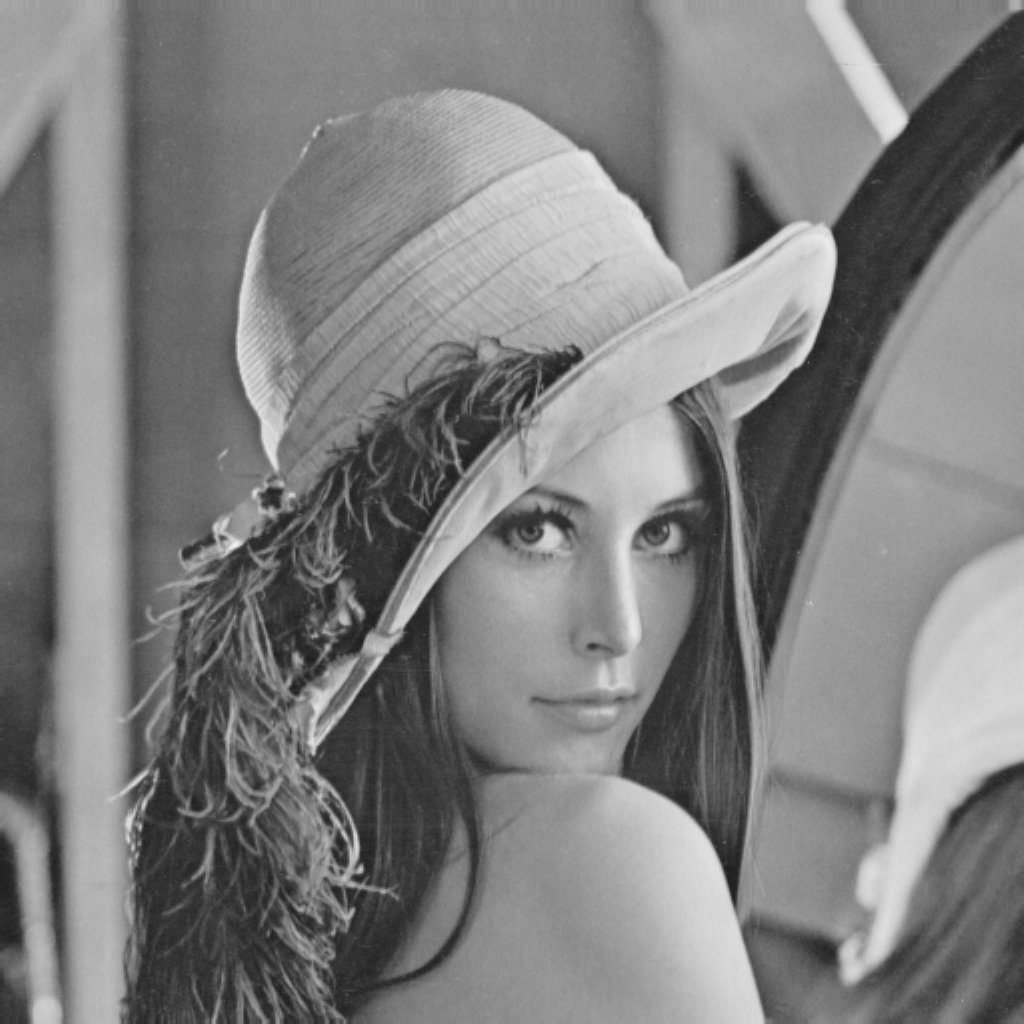
\includegraphics[width=7cm]{images/bilineare-interpolation-final/bip-scaled-2.jpg}
	\caption{Resampling anhand bilinearer Interpolation und Skalierung um Faktor 2.0}
	\label{fig:resultResamplingBilinearInterpolation-2.0}
\end{figure}

\begin{figure}[H]
	\centering
	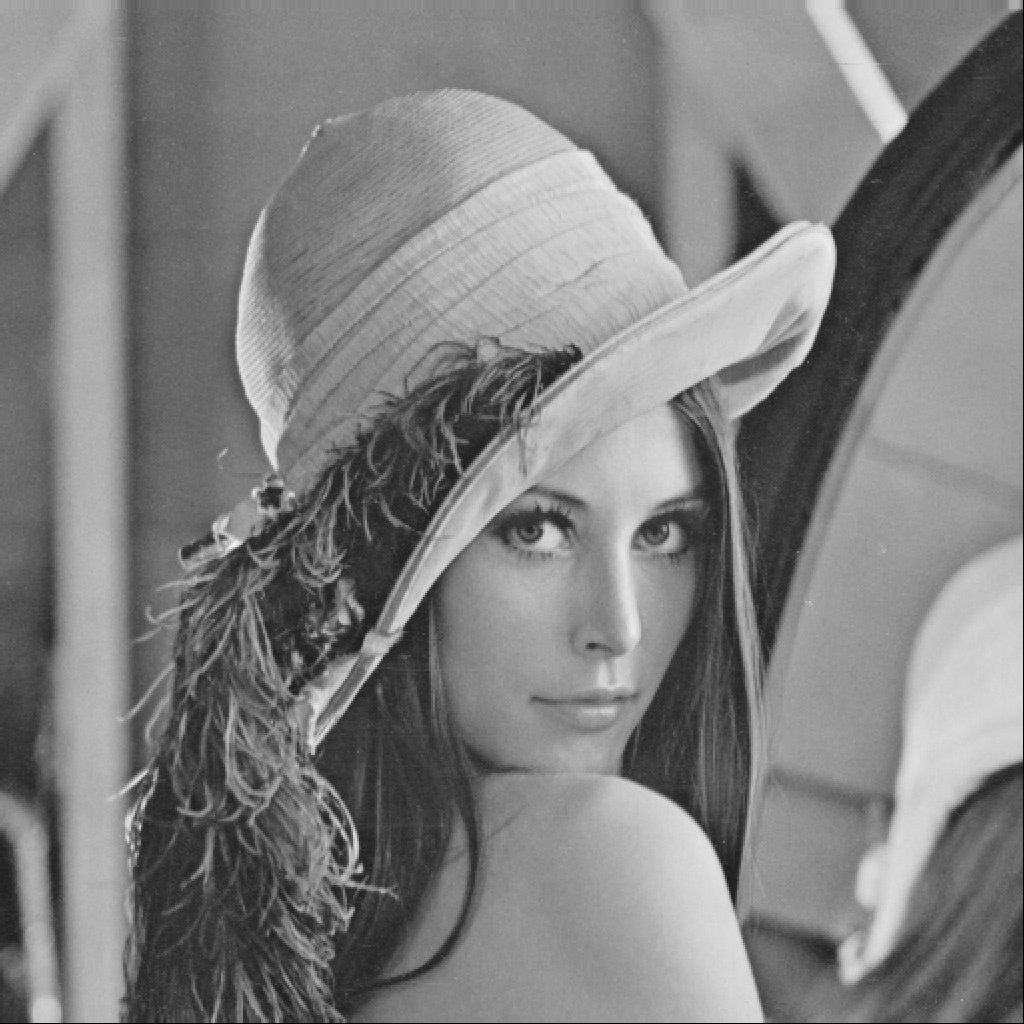
\includegraphics[width=7cm]{images/bilineare-interpolation-final/nn-scaled-2.jpeg}
	\caption{Resampling anhand Nearest Neighbor Interpolation und Skalierung um Faktor 2.0}
	\label{fig:resultResamplingNNInterpolation-2.0}
\end{figure}

\begin{figure}[H]
	\centering
	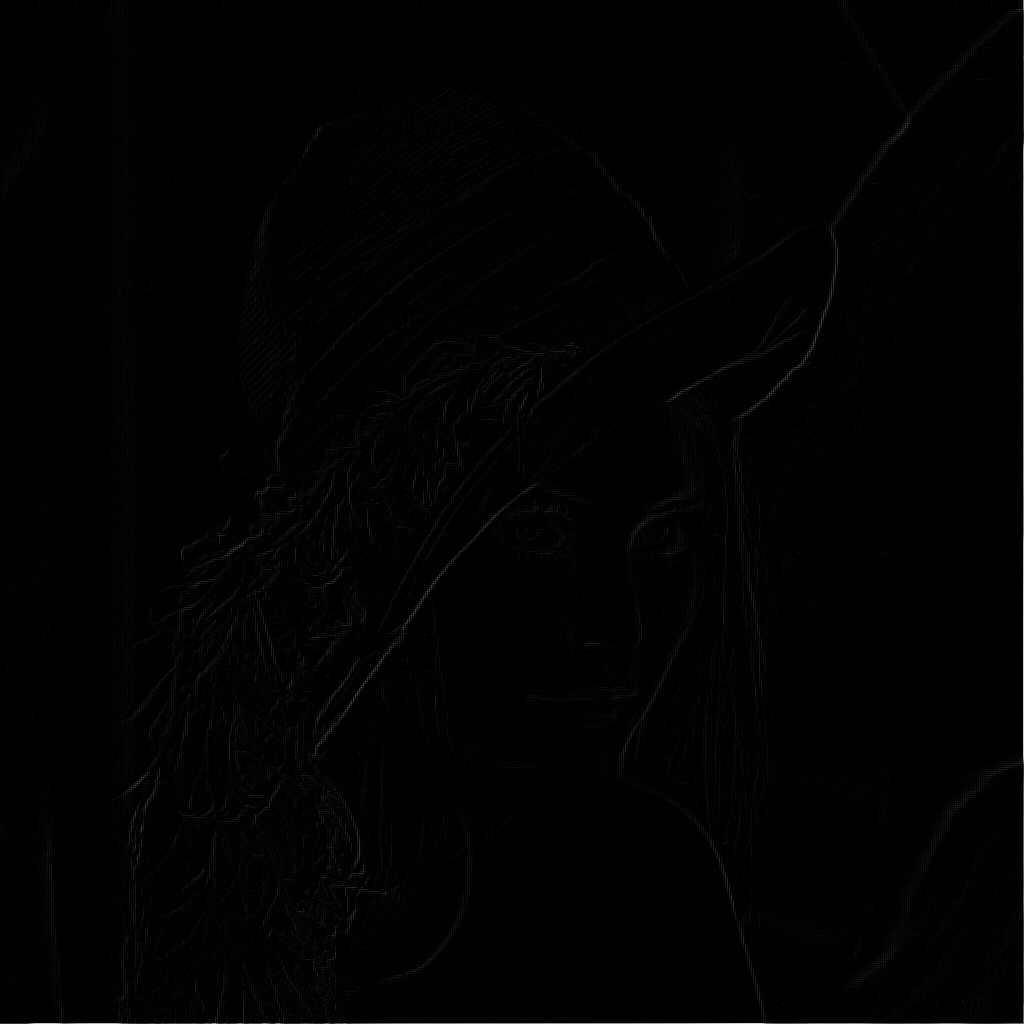
\includegraphics[width=10cm]{images/bilineare-interpolation-final/differenz-bilinear-2.jpg}
	\caption{Differenzbild generiert aus Nearest Neighbor und bilinearer Interpolation}
	\label{fig:resultResamplingDifference}
\end{figure}

Figure 3 visualisert die Differenz zwischen den Testbildern der Nearest Neighbor und der bilinearen Interpolation. Bei näherer Betrachtung sieht man, dass sich an den Umrissen von Lena im Bild weiße Ausprägungen wiederfinden. Diese weißen skalaren Werte bedeutet, dass es hier zwischen den zwei Bildern Unterschiede gibt. Dies verdeutlicht, dass die NN Interpolation aufgrund keiner Neuberechnung der Werte, diese nicht so gut wiedergibt. Diese Unterschiede in den skalaren Werten ergeben sich daraus, dass die bilineare Interpolation aufgrund der Verwendung des gewichteten Mittelwerts von 4 Pixeln einen ähnlicheren skalaren Wert ergibt, als bei der NN Interpolation.


\subsubsection{Implementierung Checker-Board}

Das Checkerboard wurde innerhalb des Resample Filters implementiert und bedient sich der neuberechneten Werte. Die skalaren Werte, die aus den beiden Methoden berechnet werden, werden in einem neuen Array für das skalierte Checkerboard abwechselnd eingetragen.\\

\begin{figure}[H]
	\centering
	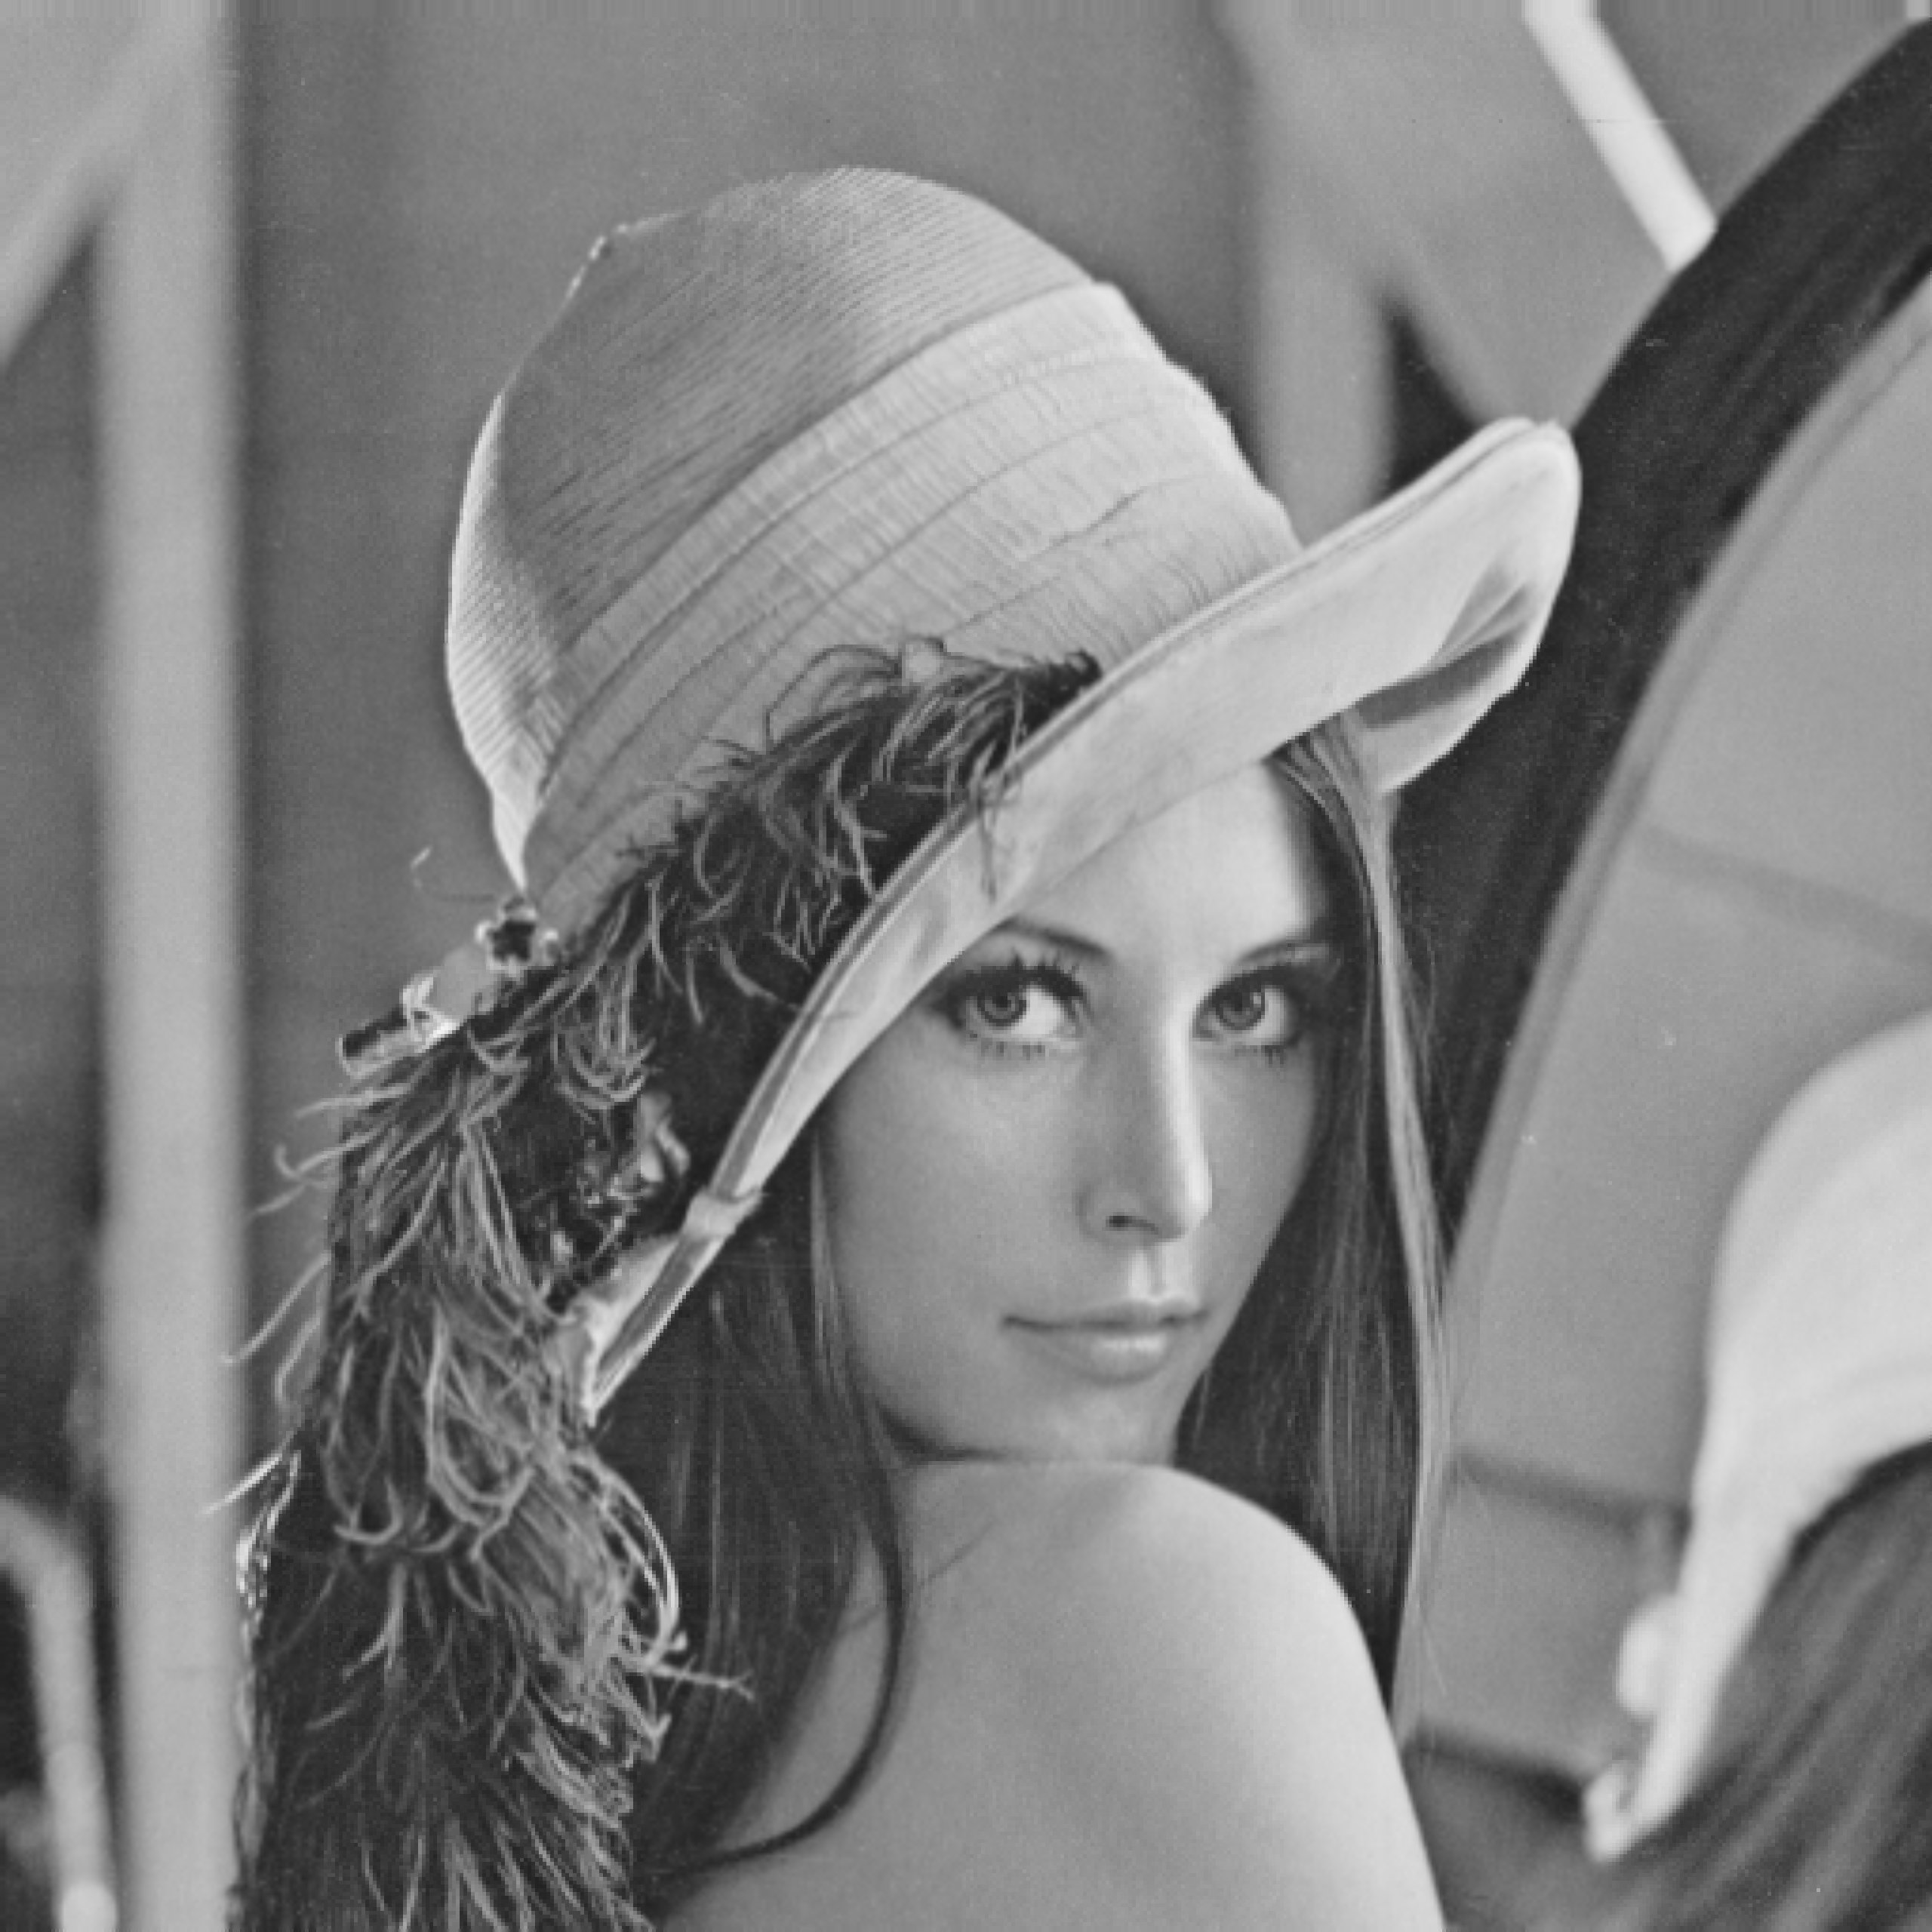
\includegraphics[width=7cm]{images/bilineare-interpolation-final/scaled-img-checkerboard.jpg}
	\caption{Checkerboard mit Nearest Neighbor und bilinearer Interpolation}
	\label{fig:resultCheckerboard}
\end{figure}

Da sich die beiden Interpolationsstrategien nur bei genauer Betrachtung erkennen lassen, wurde ein Teil des Checkerboards vergrößert (siehe Figure 5). Bei den Segment links unten und rechts oben erkennt man, das das Bild hier pixeliger ist (NN).

\begin{figure}[H]
	\centering
	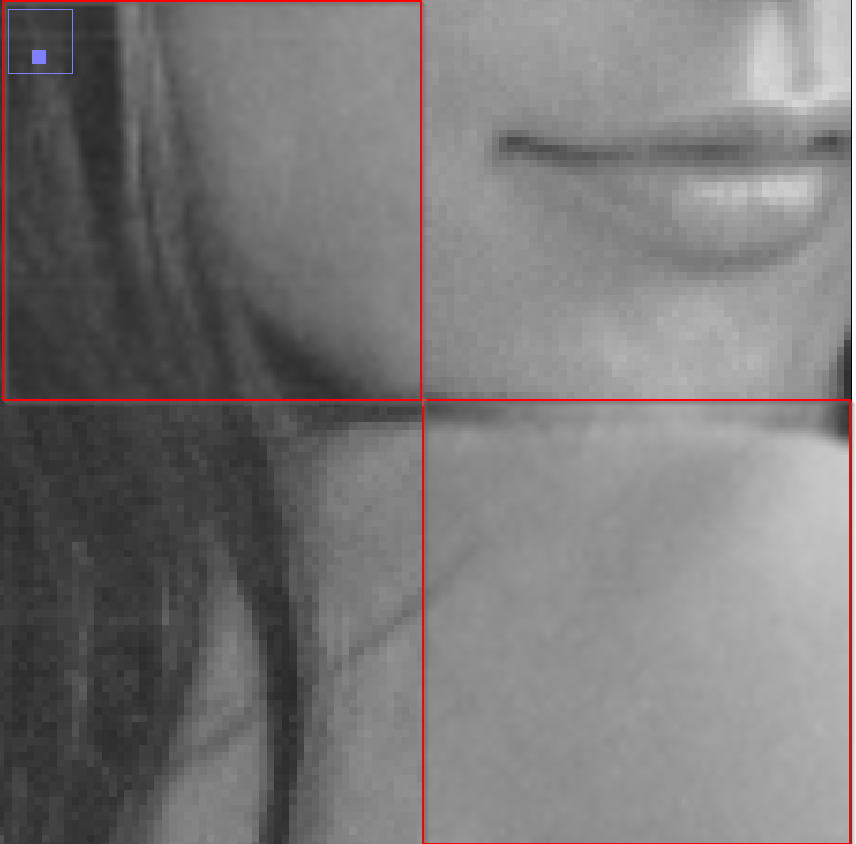
\includegraphics[width=7cm]{images/bilineare-interpolation-final/scaled-img_checkerboard-NN-BI-boxes.png}
	\caption{Checkerboard Vergrößerung}
	\label{fig:resultCheckerboardZoom}
\end{figure}

\textit{Charakterisierung der Interpolationsstrategien}

Die Nearest Neighbor Interpolation bezieht sich in ihrer Berechnung auf keinen neuen skalaren Wert. Es werden jeglich die benachbarten Pixel geprüft, und der Wert der am Nähesten ist, für den neuen Pixel herangezogen. Die Neuzuweisung schlägt sich auf die Bildqualität wieder, dieser wird bei einer Skalierung pixeliger bzw. kantiger. Dieser Effekt tritt dann sehr deutlich auf, wenn das Bild zuerst stark verkleinert und anschließend wieder vergrößert wird (0.5 ; 10).

Theoretische Überlegung: Da bei dieser Strategie kein komplexer Algorythmus verwendet wird und nur eine Neuzuweisung statt - berechnung stattfindet, ist dieser schneller als die andere Strategie.

Die bilineare Interpolation hingegen bedient sich auch der benachbarten Pixel, berechnet jedoch auf Basis dieser den gewichteten Mittelwert. Dieser Wert ist ähnlicher als zum Beispiel die Zuweisung der NN Interpolation und resuliert daher in einer besseren Bildqualität. 

Theoretische Überlegung: Aufgrund der Verwendung eines komplexeren Algorythmus ist die Laufzeit bei diesem auch länger.

 \subsection{Klassifizierung mittels Kompression}
\subsubsection{Klassifizierung von Texten}

\textbf{Idee}

Aus Texten in 8 verschiedenen Sprachen soll mittels Kompression eine Klassifizierung stattfinden. Zur Testzwecken wurden folgende Datensätze als \textit{ *.txt}  Datein in bosnisch, deutsch, englisch, spanisch, französisch, niederländisch, polnisch und ungarisch aufbereitet:

\begin{itemize}
	\item Abstract einer wissenschaftlichen Arbeit. Diese hat den Vorteil, dass es eine deutsche und englische Übersetzung gibt. Alle weiteren Sprachen wurden aus der englischen Version mittels \textit{google translate} generiert.
	\item Wörterbuch mit 10000 deutschen Wörtern. Dieser Datensatz wurde mittels \textit{google translate} in die anfangs erwähnten Sprachen übersetzt.
	\item Die erste Seite der Datenschutzrichtlinien von Facebook. Da die Datenschutzrichtlinien in sämtlichen Sprachen abrufbar sind, konnte für alle Sprachen ein passender Datensatz gefunden werden.
	\item Die erste Seite der Datenschutzrichtlinien von Google. Auch hier waren Daten in allen Sprachen verfügbar.
	\item Ein Witz der aus dem deutschen mittels \textit{google translate} in alle anderen Sprachen übersetzt wurde.
\end{itemize}

Zur Weiterverarbeitung wurden den Sprachen Nummern zugeordnet. Folgende Liste gibt die Zuordnung wieder:

\begin{itemize}
	\item 1 = bosnisch
	\item 2 = deutsch
	\item 3 = englisch
	\item 4 = spanisch
	\item 5 = französisch
	\item 6 = niederländisch
	\item 7 = polnisch
	\item 8 = ungarisch
\end{itemize}

Da nach einer Übersetzung die Texte in verschiedenen Sprachen nicht dieselbe Anzahl an Buchstaben beinhalten, variiert auch die Dateigröße. Dies könnte eventuell rechnerisch berücksichtigt werden. Es wurde jedoch die Variante gewählt, die letzten Buchstaben jedes langen Textes zu ignorieren und so eine einheitliche Länge des Textes zu gewährleisten. Dies wurde mittels eines shell-Skripts erreicht, welches nur die ersten $n$ Bytes eines Files speichert. So konnte für jeden Text eine Datei erzeugt werden die in allen Sprachen den selben Speicherbedarf hat. Der Verlust der letzten Byte ist bei einer Klassifizierung unwesentlich. 

\lstinputlisting[frame=single,language=MATLAB,breaklines=true]{../cutData.sh}

Nach einer solchen Normierung der Texte können diese nun miteinander verglichen werden. Dazu wurde ein Programm in \textit{Octave} geschrieben (siehe Listing \ref{fig: calculateMatrixOctaveCode}  , welches die Texte der einzelnen Datensätze miteinander vergleicht und in einer Matrix darstellt. Eine qualitativ hochwertige Aussage, ob die Ergebnisse statistische Aussagekraft haben, kann mit $5$ Datensätzen nicht getroffen werden. Es ist aber sicherlich ein Trend erkennbar.

\begin{table}[H]
  \centering
  \begin{tabular}{| l | c | c | c | c | c |}
	\hline
	Datensätze & Abstract & Dictionary & Facebook & Google & Witz \\ 
    \hline
    Abstract &
    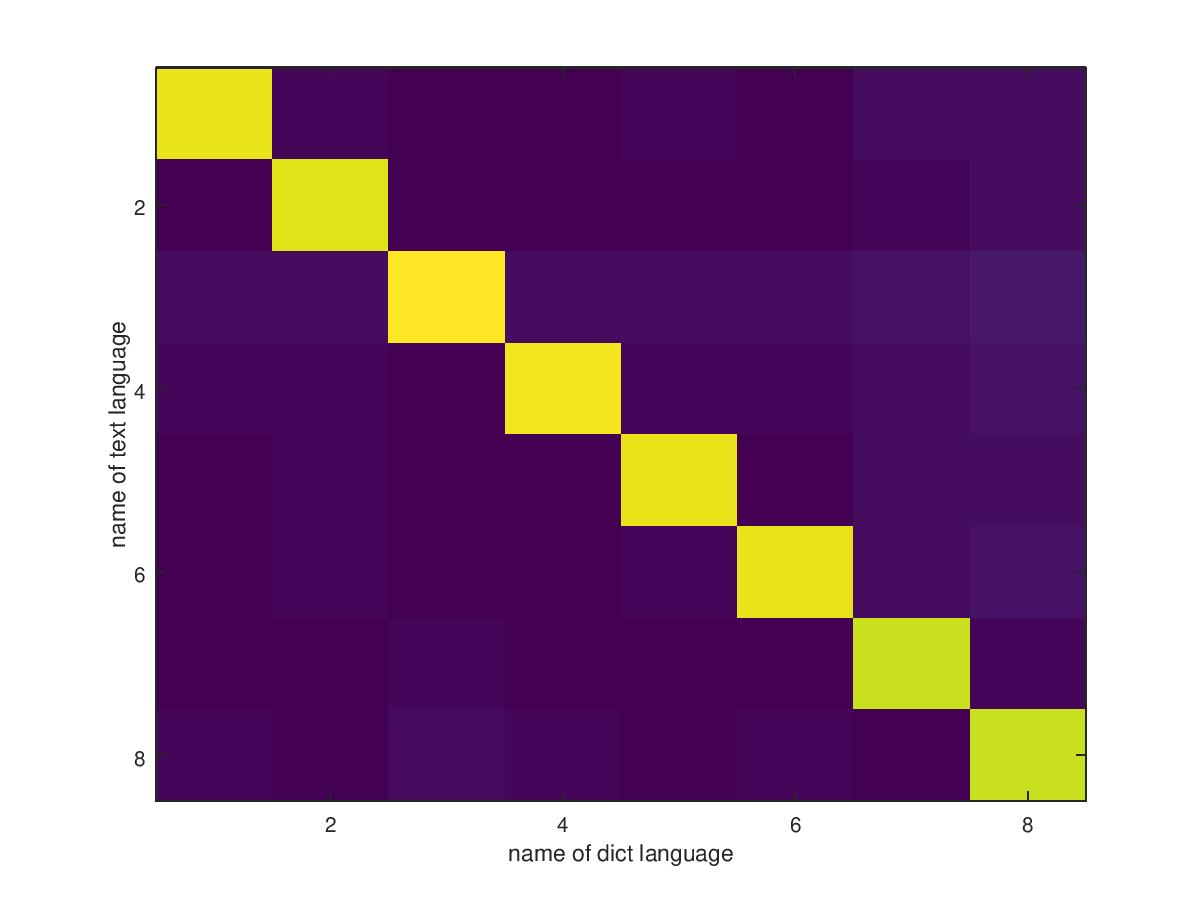
\includegraphics[width=2.5cm]{../images/abstractData/abstractData.jpg} &
    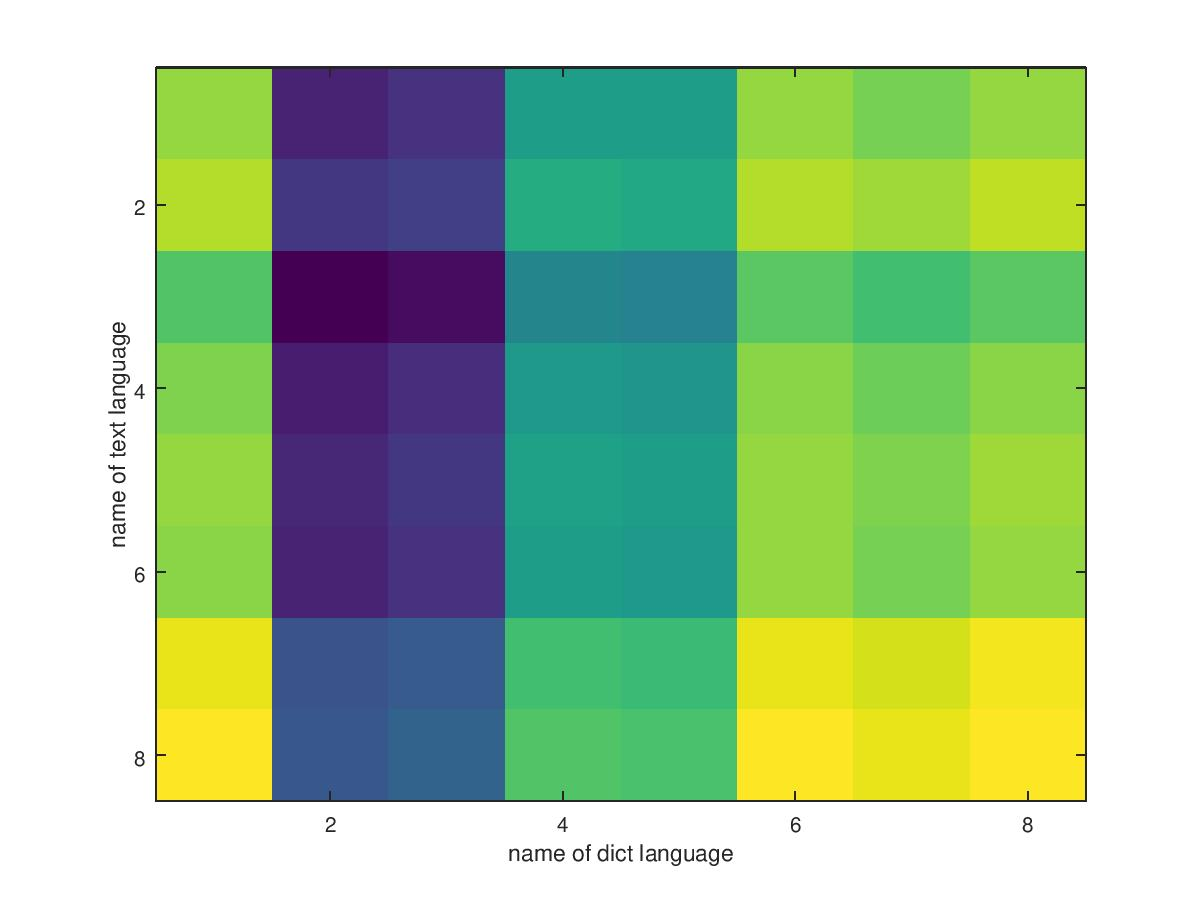
\includegraphics[width=2.5cm]{../images/abstractData/dictData.jpg} &
    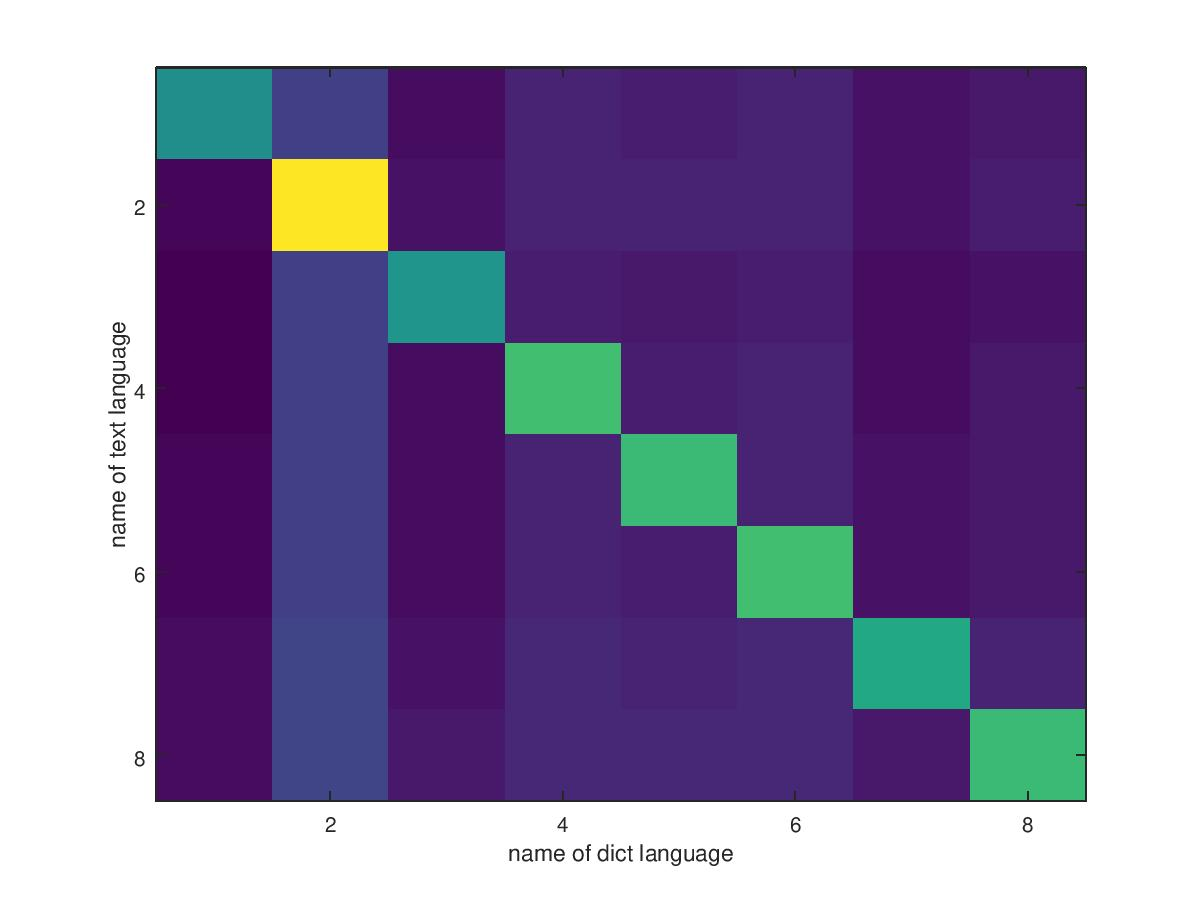
\includegraphics[width=2.5cm]{../images/abstractData/facebookData.jpg} &
    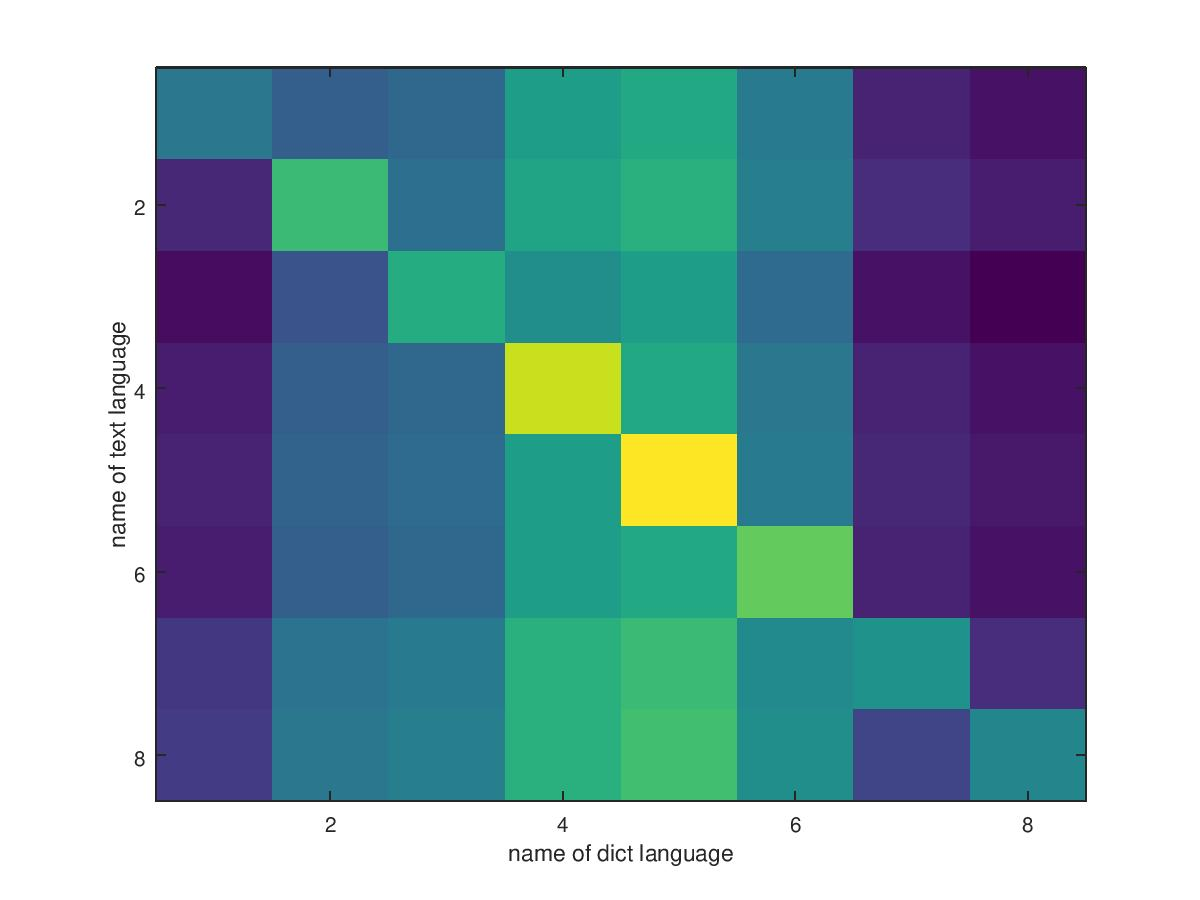
\includegraphics[width=2.5cm]{../images/abstractData/googleData.jpg} &
    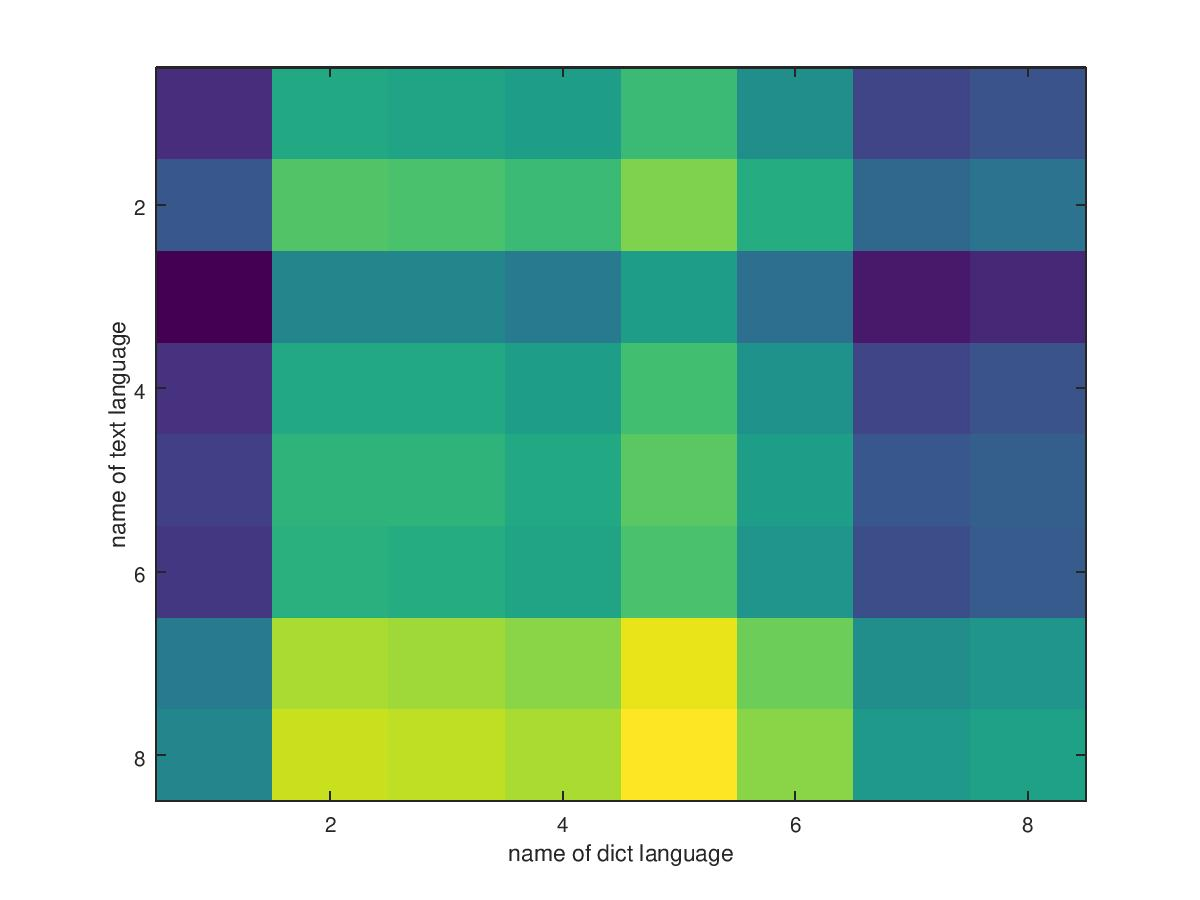
\includegraphics[width=2.5cm]{../images/abstractData/witzData.jpg} \\
    \hline
    Dictionary &
    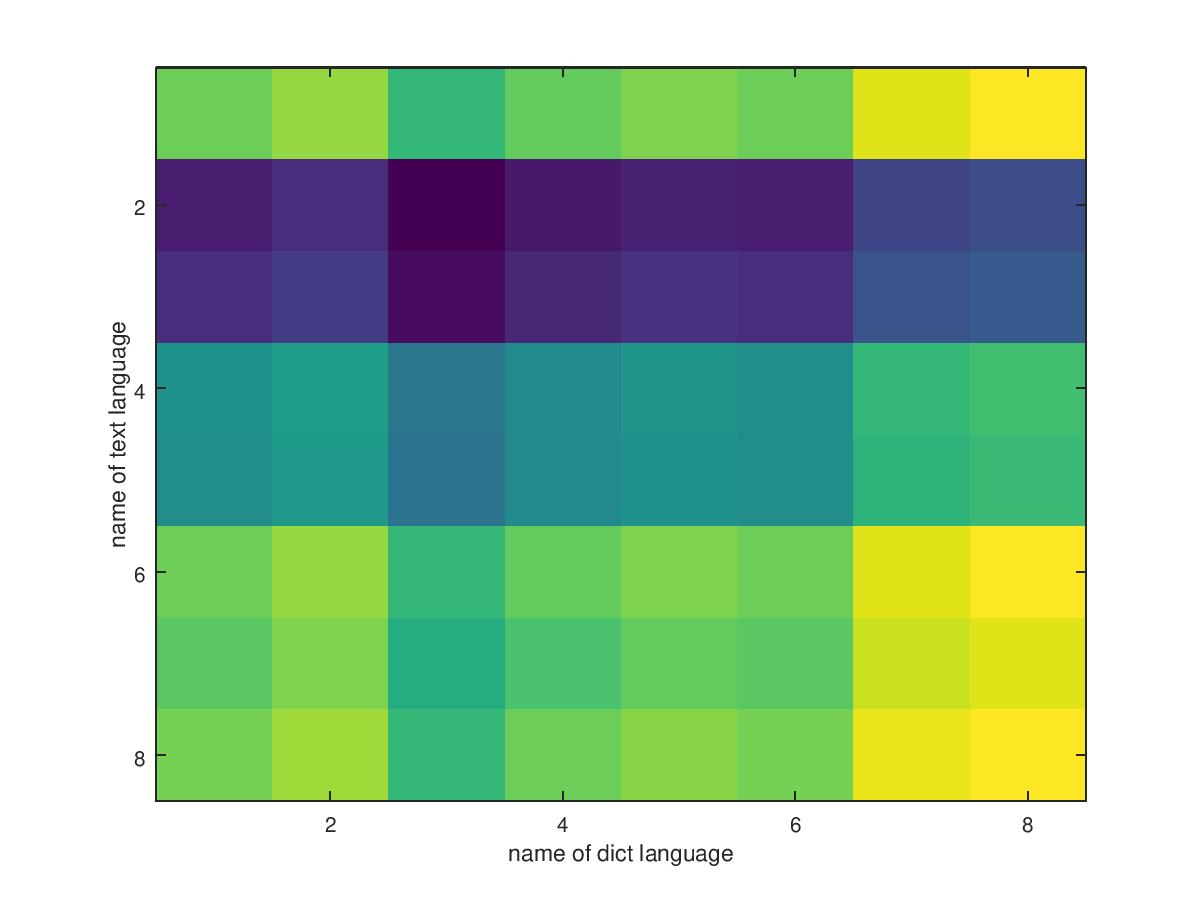
\includegraphics[width=2.5cm]{../images/dictData/abstractData.jpg} &
    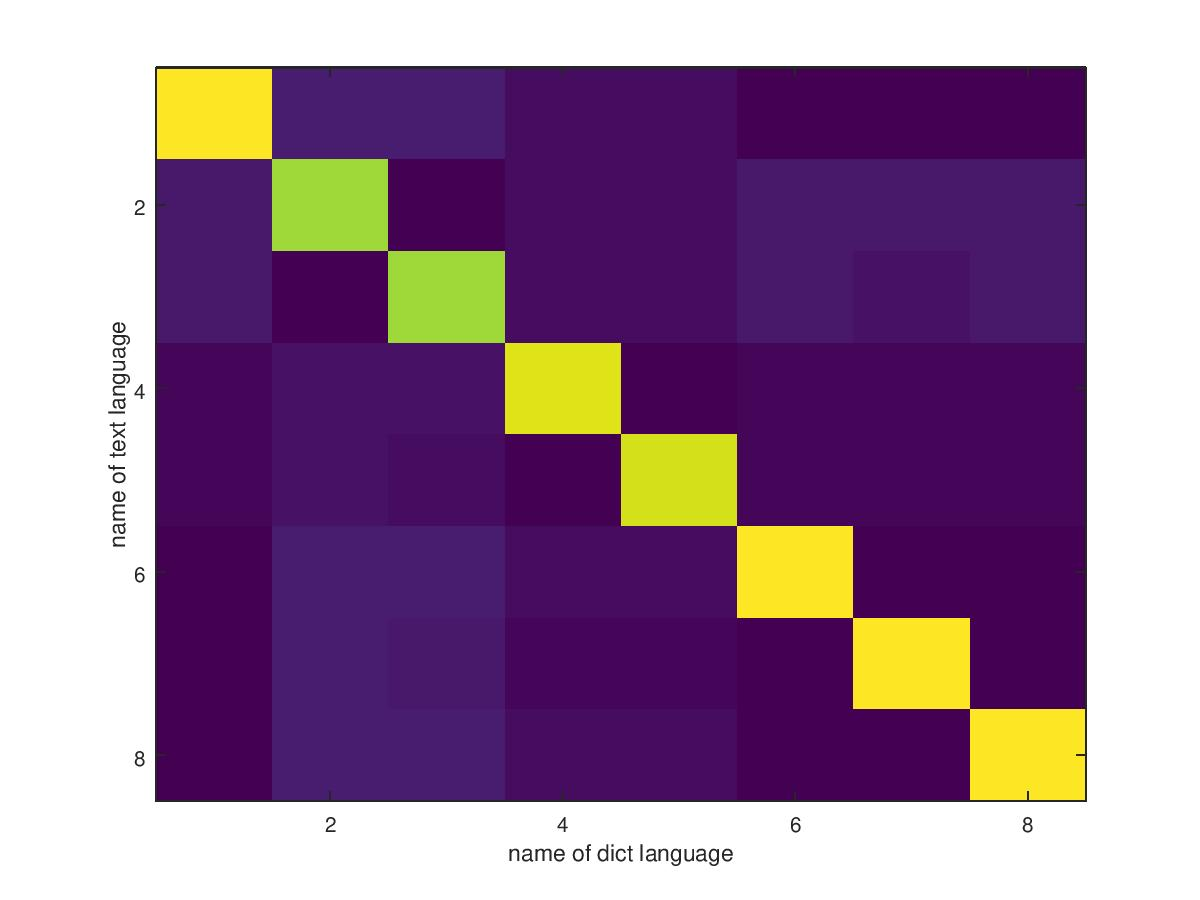
\includegraphics[width=2.5cm]{../images/dictData/dictData.jpg} &
    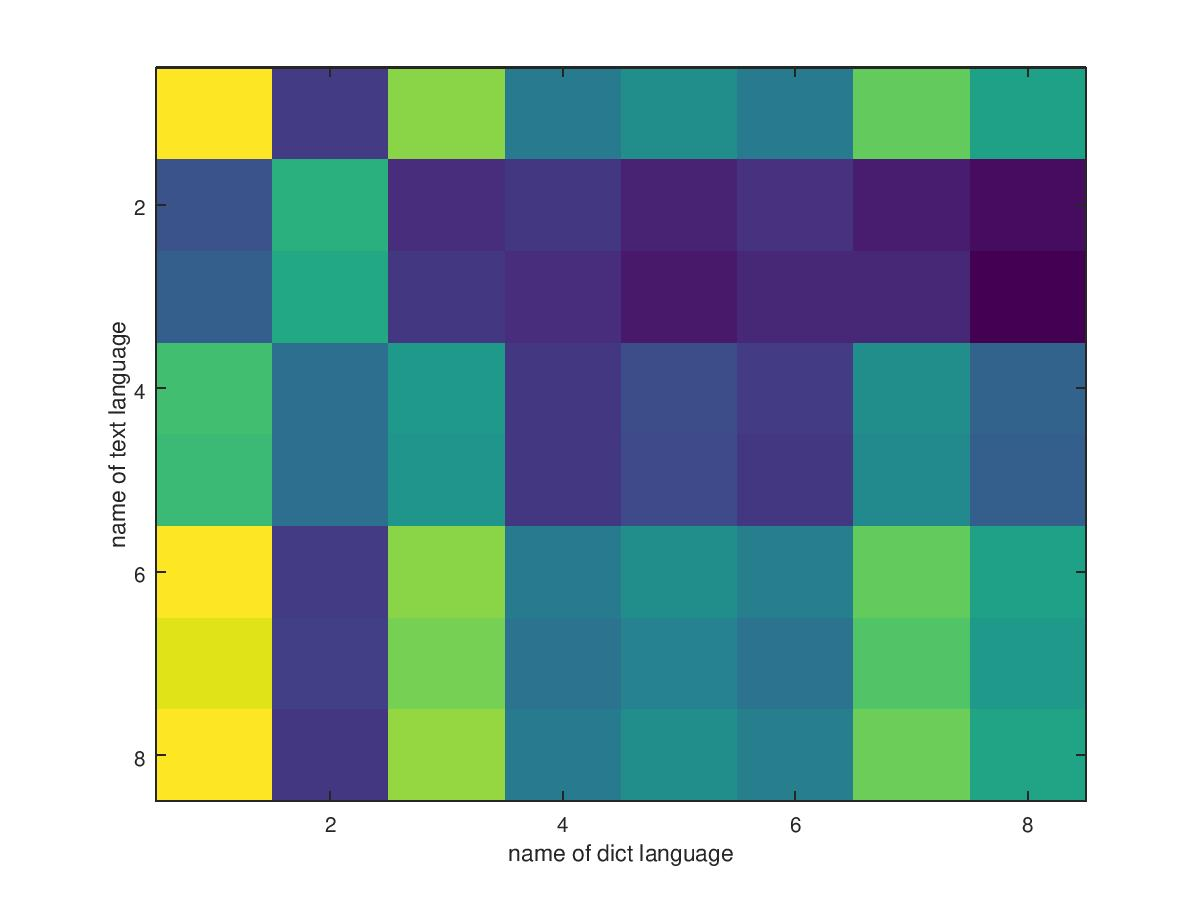
\includegraphics[width=2.5cm]{../images/dictData/facebookData.jpg} &
    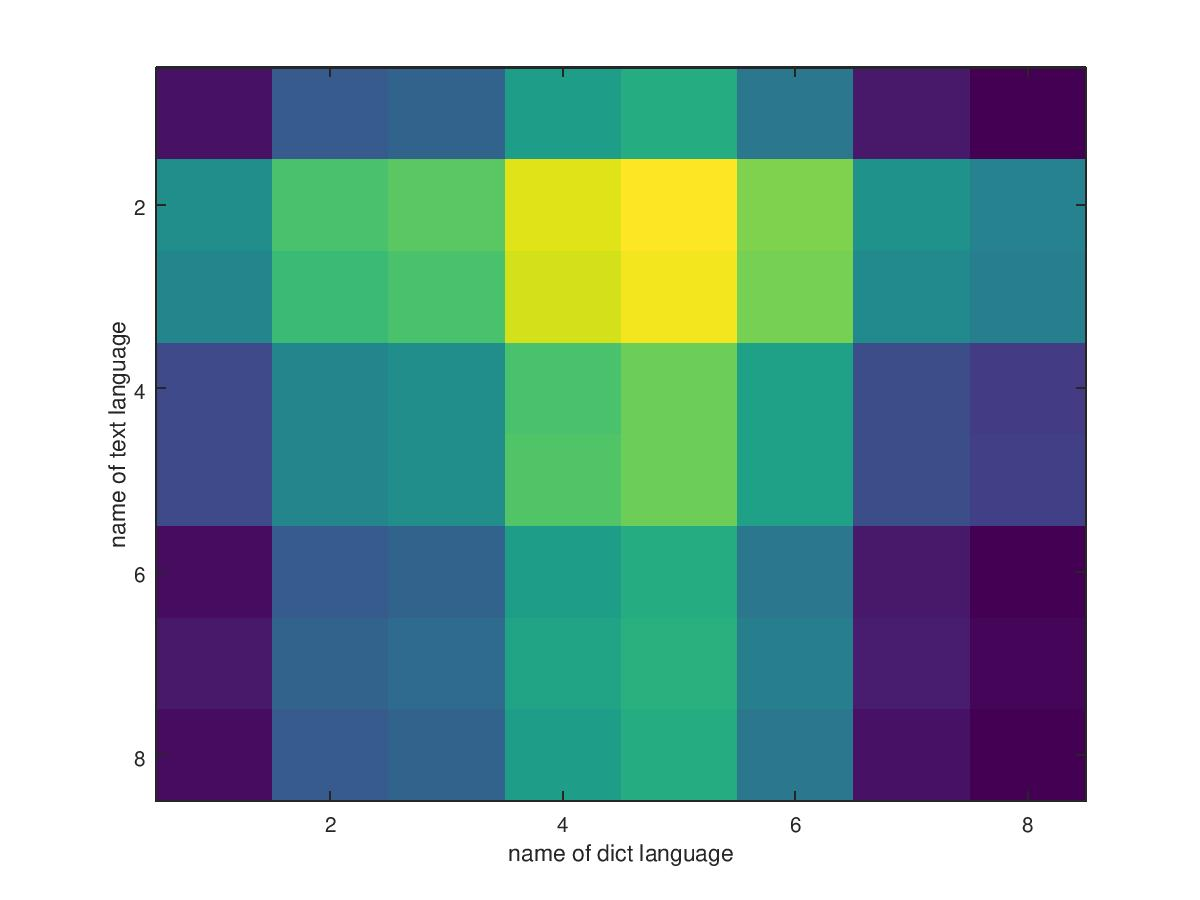
\includegraphics[width=2.5cm]{../images/dictData/googleData.jpg} &
    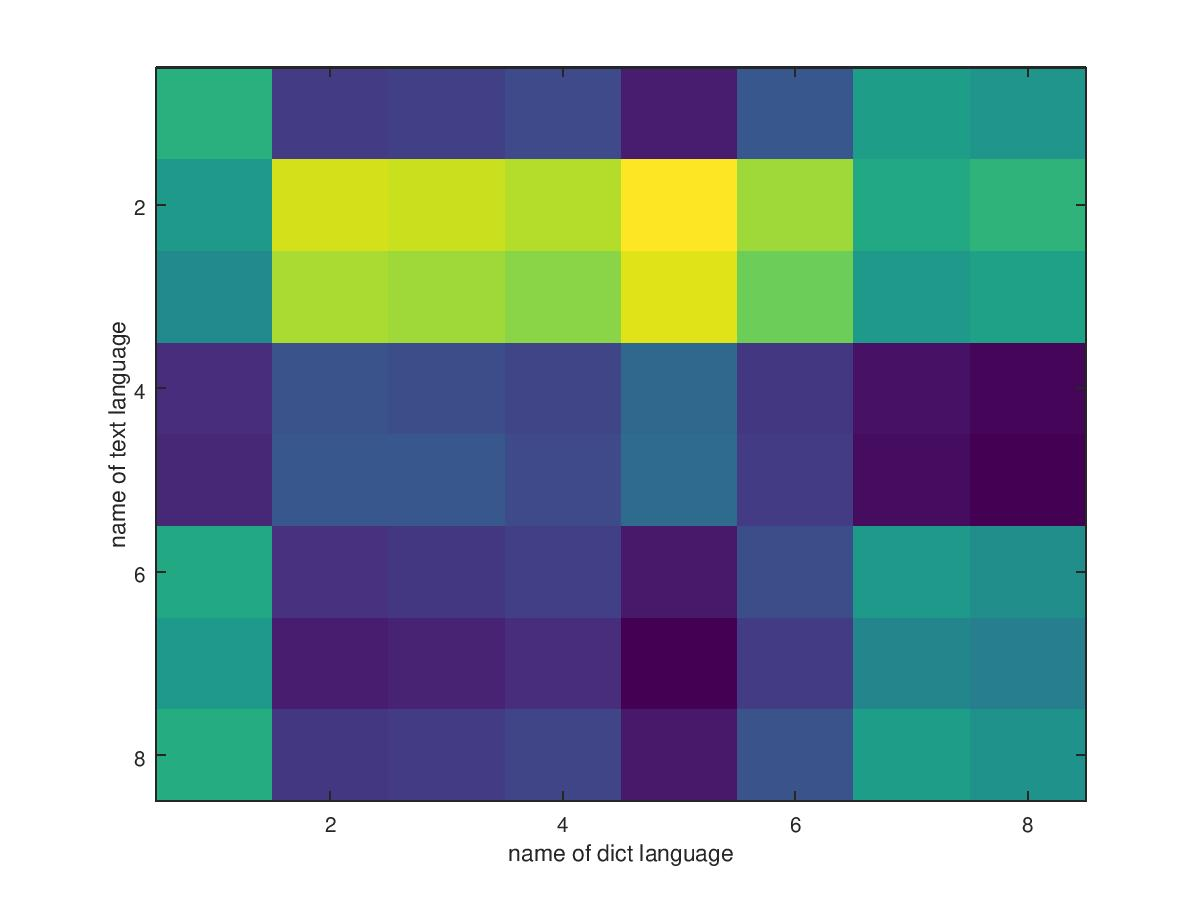
\includegraphics[width=2.5cm]{../images/dictData/witzData.jpg} \\   
    \hline
    Facebook &
    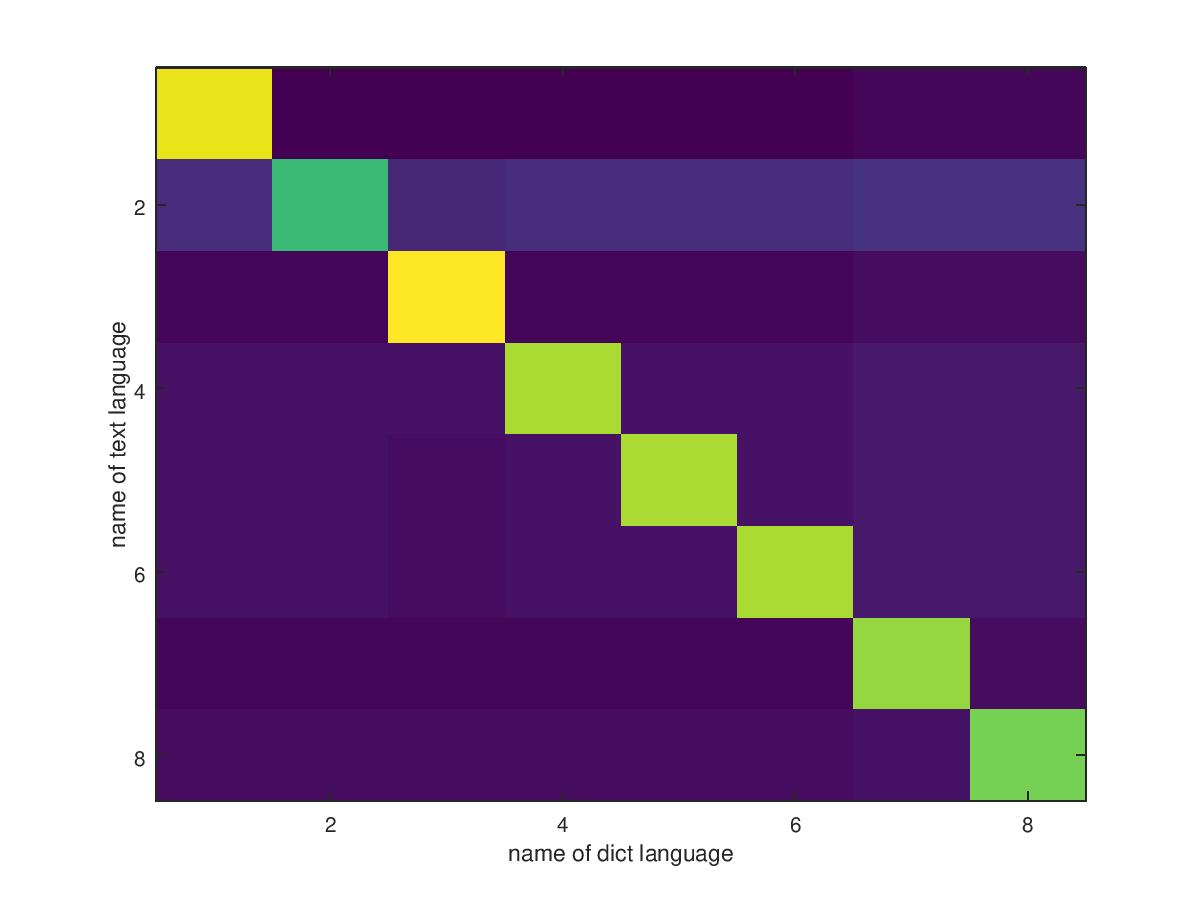
\includegraphics[width=2.5cm]{../images/facebookData/abstractData.jpg} &
    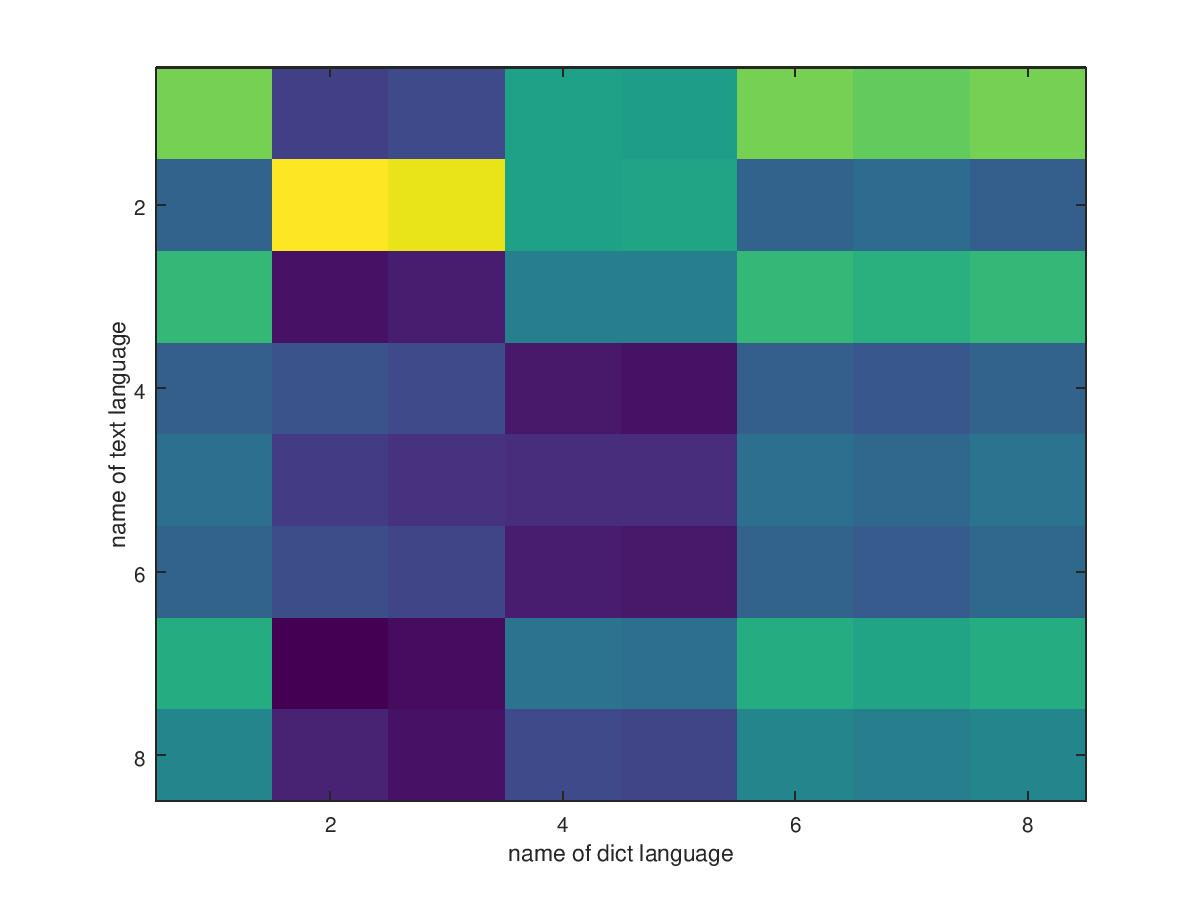
\includegraphics[width=2.5cm]{../images/facebookData/dictData.jpg} &
    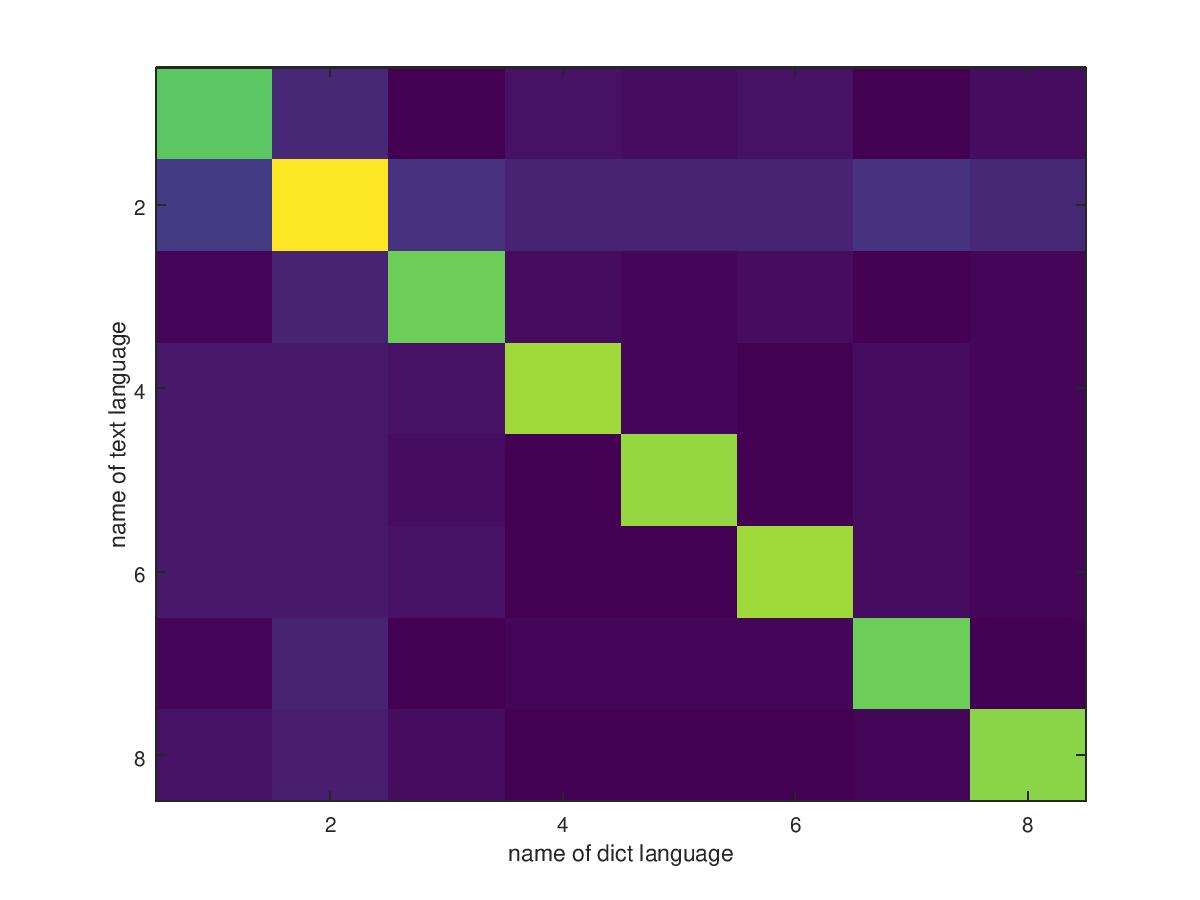
\includegraphics[width=2.5cm]{../images/facebookData/facebookData.jpg} &
    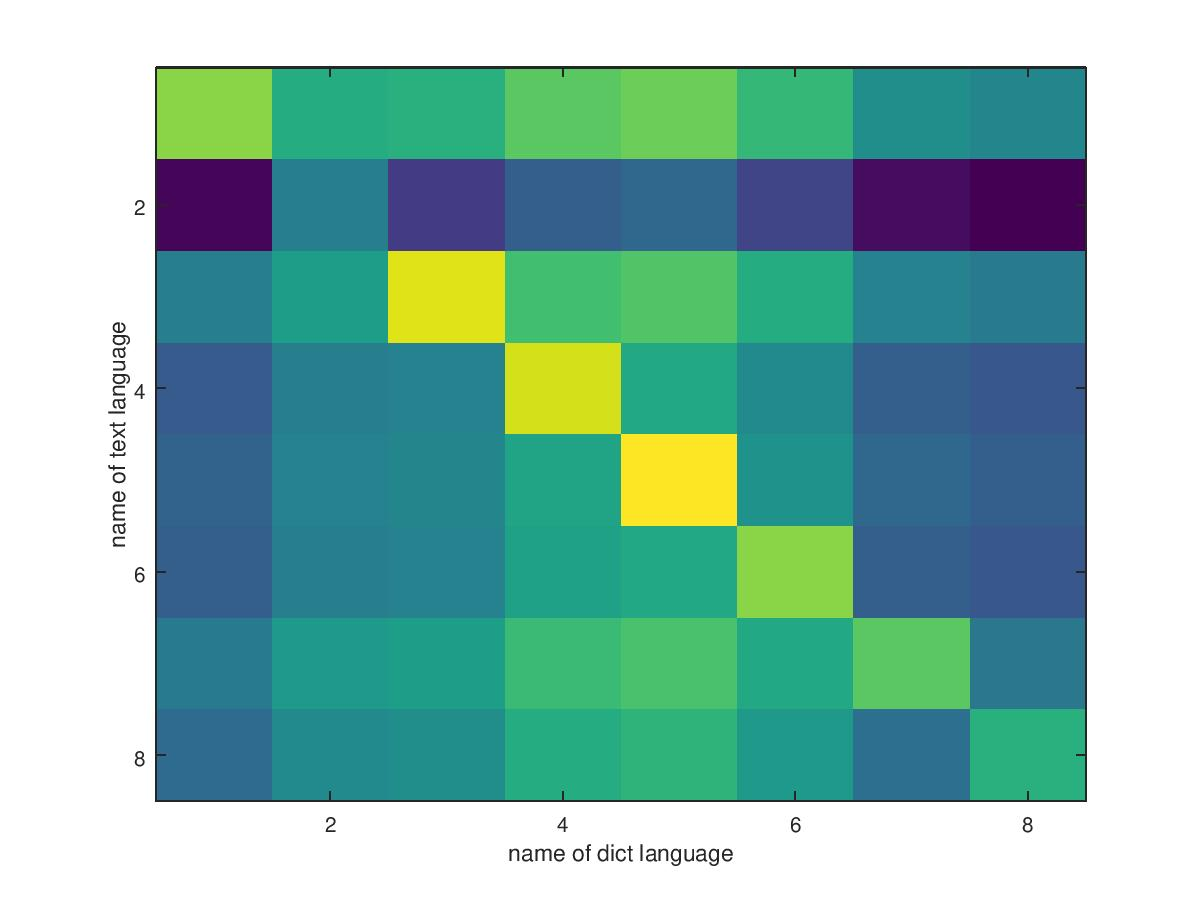
\includegraphics[width=2.5cm]{../images/facebookData/googleData.jpg} &
    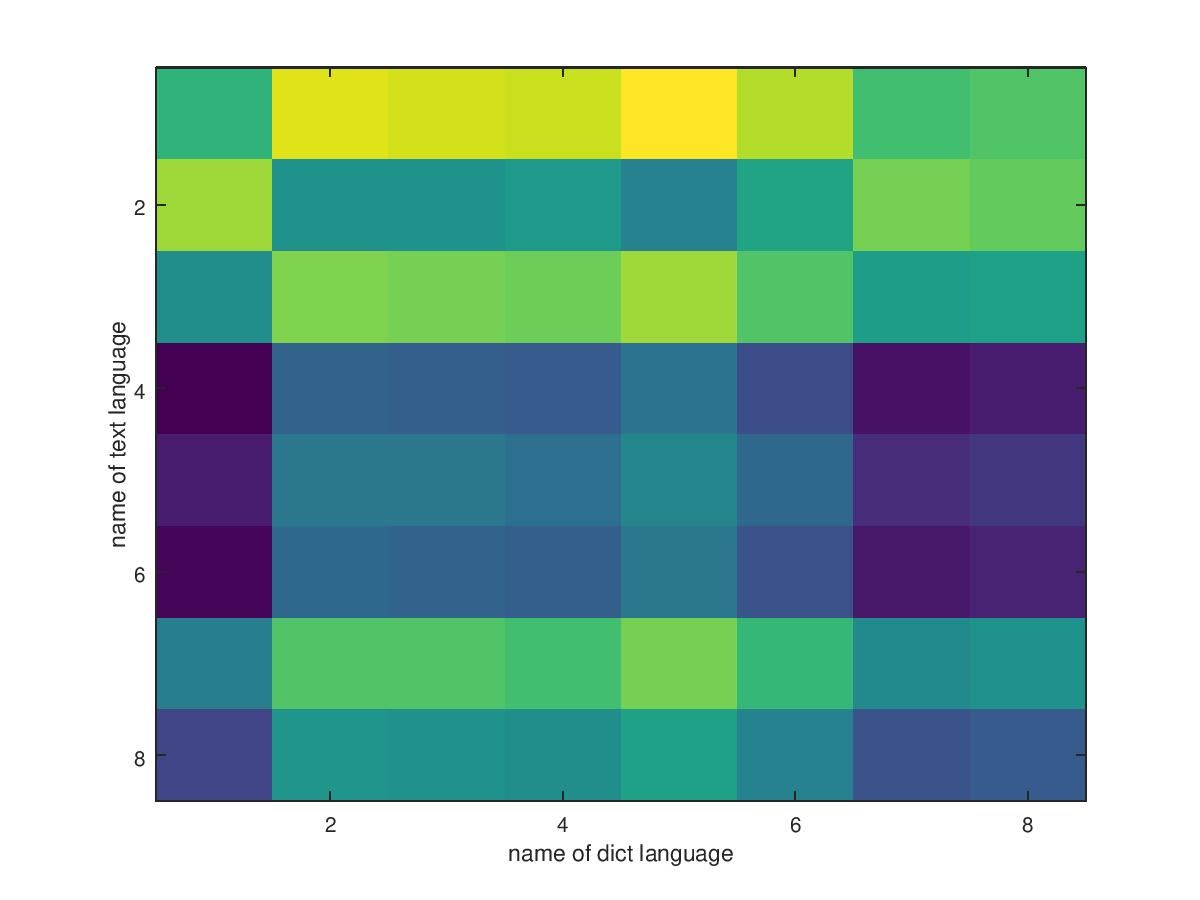
\includegraphics[width=2.5cm]{../images/facebookData/witzData.jpg} \\
    \hline
    Google &
    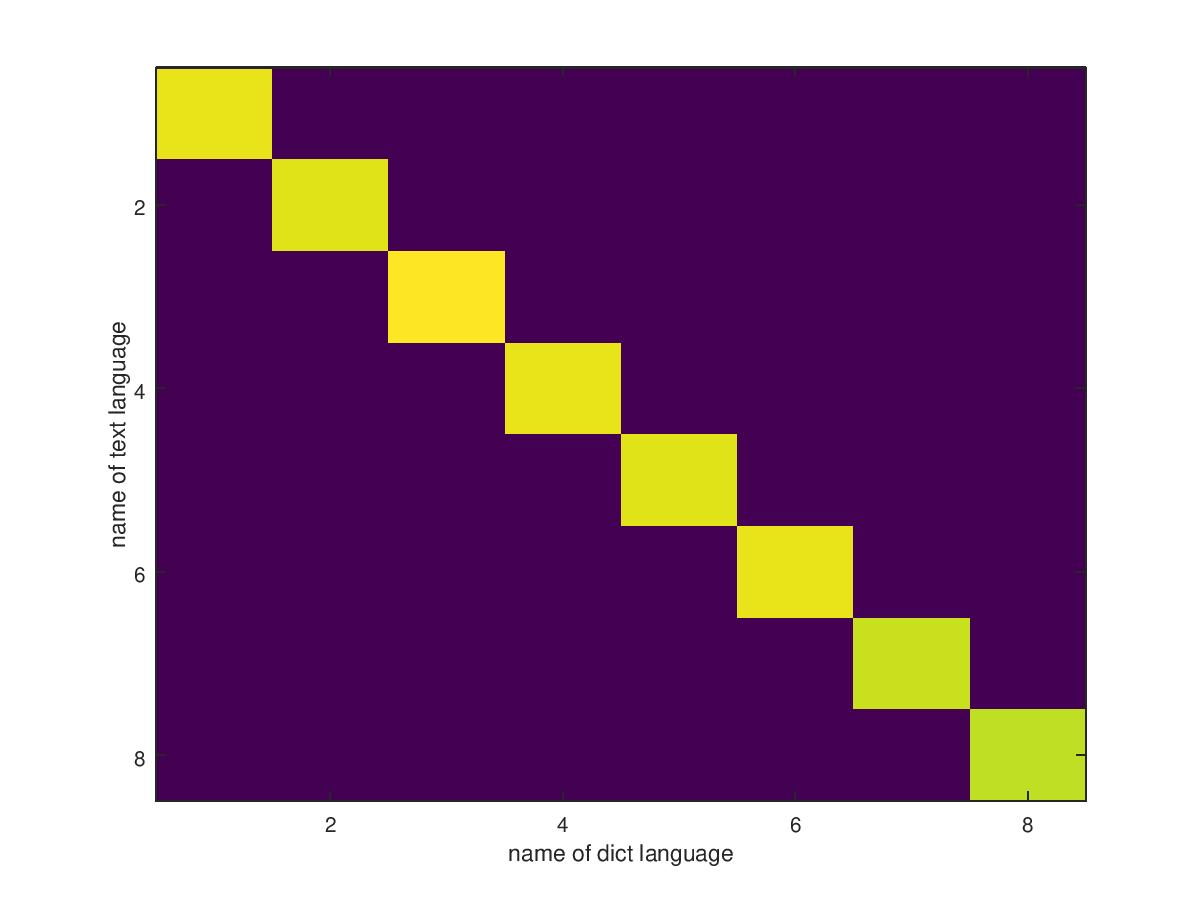
\includegraphics[width=2.5cm]{../images/googleData/abstractData.jpg} &
    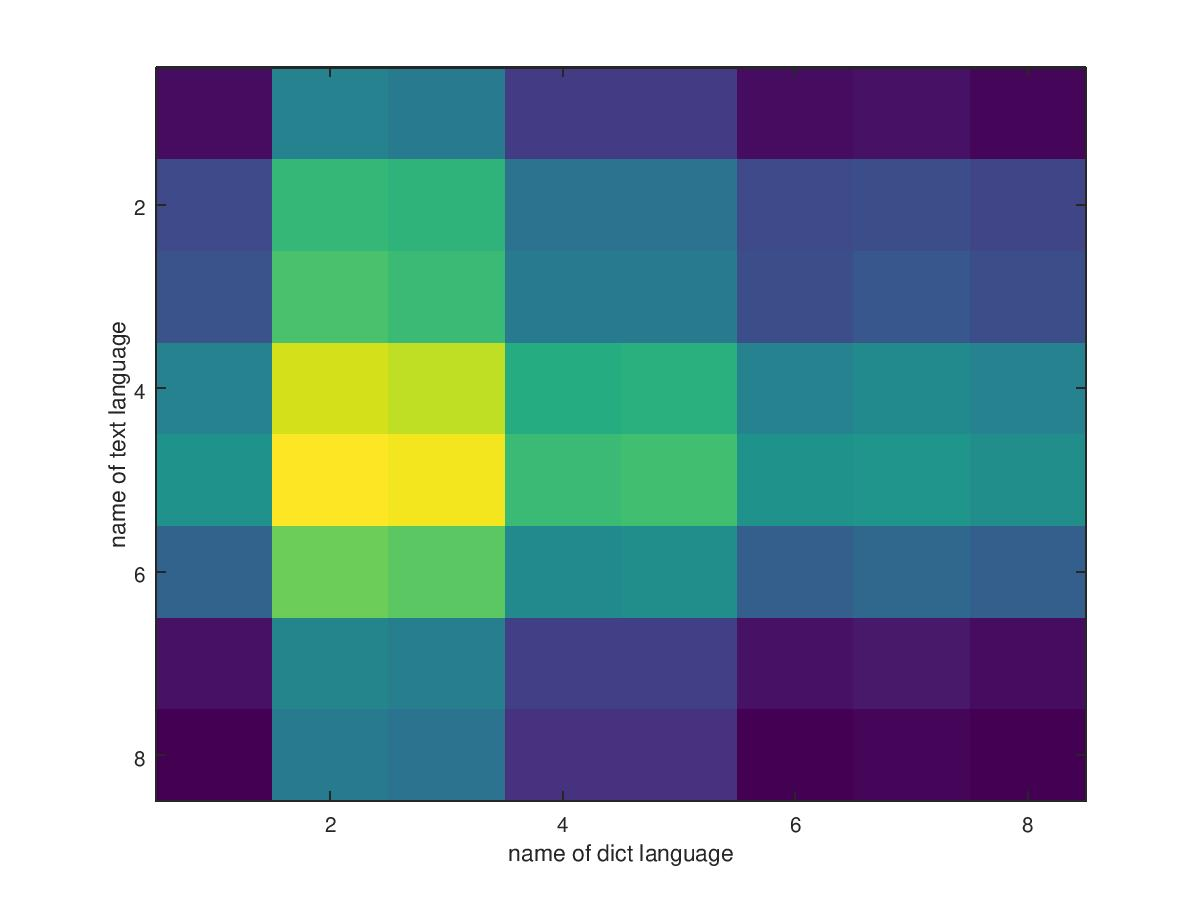
\includegraphics[width=2.5cm]{../images/googleData/dictData.jpg} &
    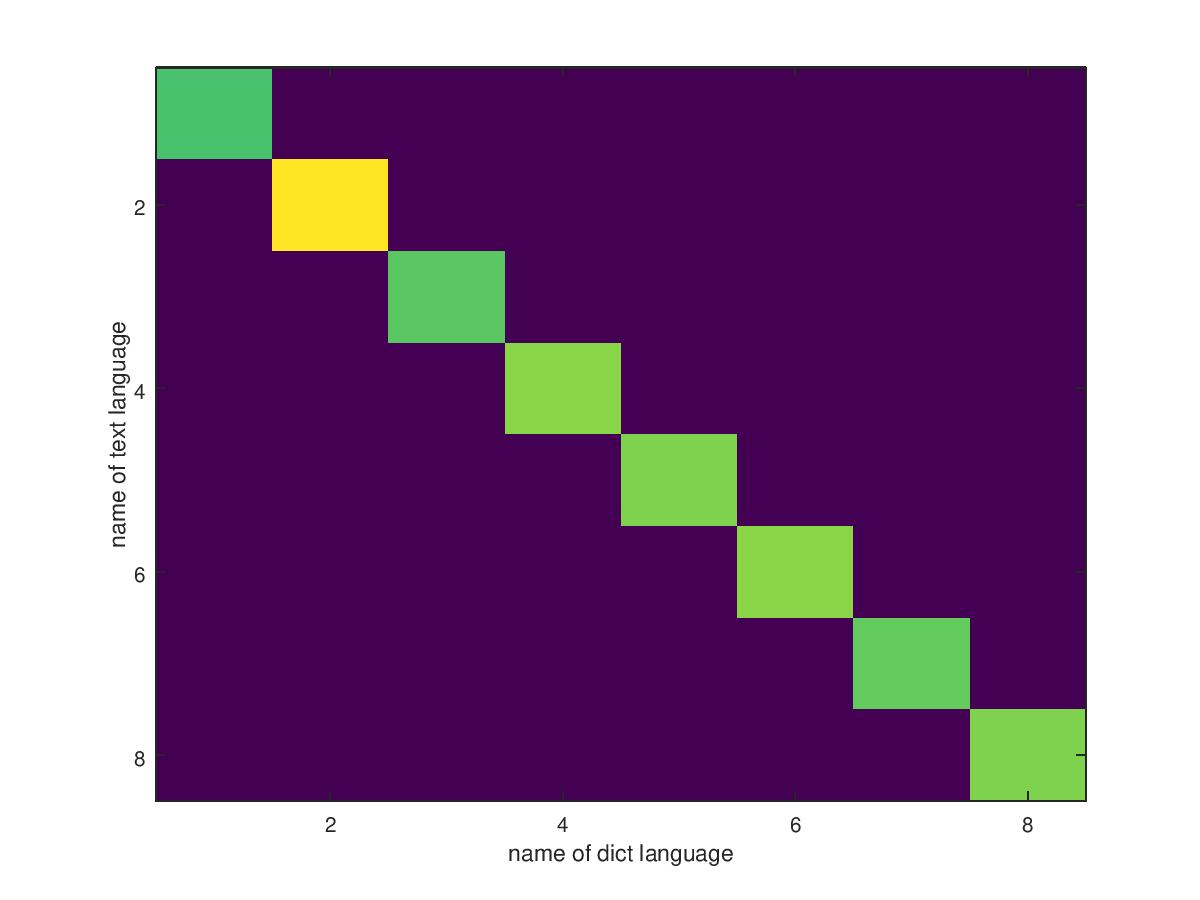
\includegraphics[width=2.5cm]{../images/googleData/facebookData.jpg} &
    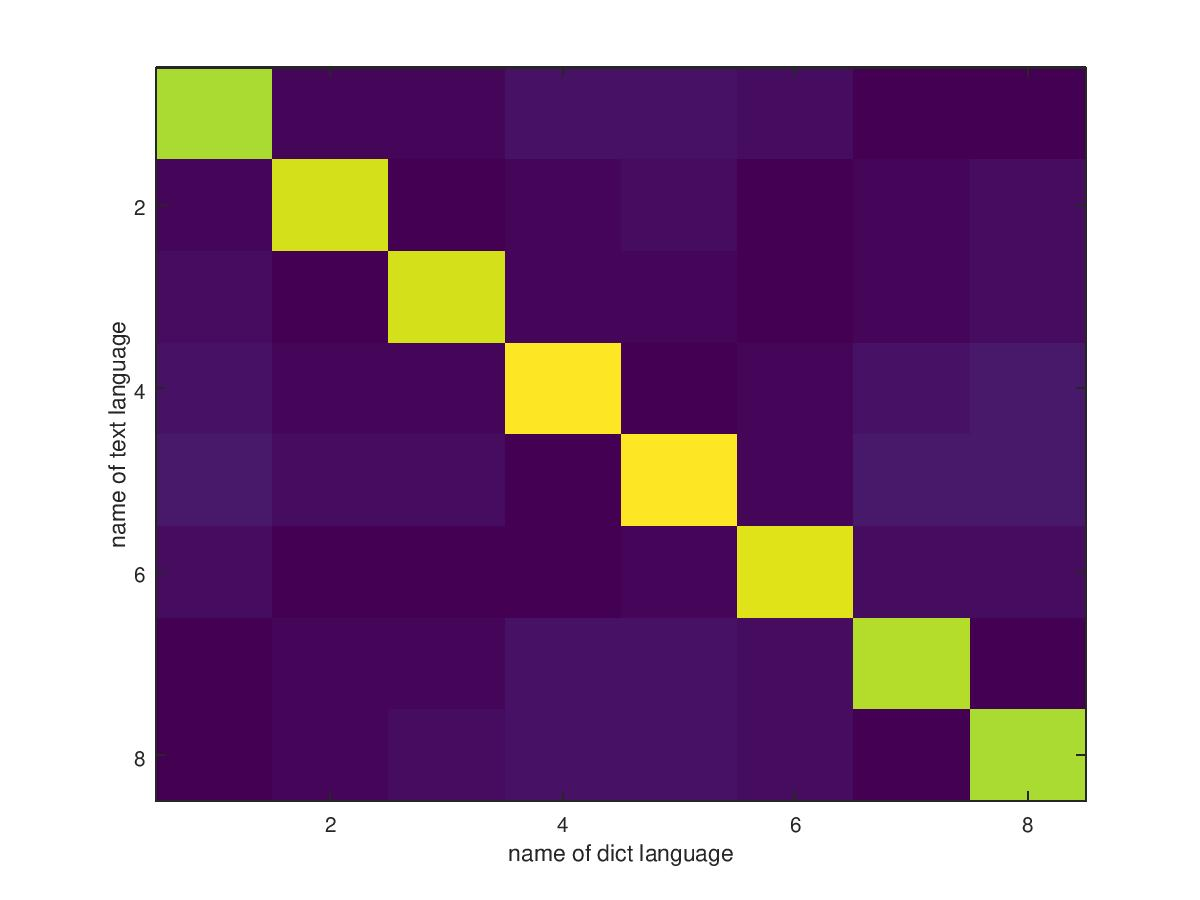
\includegraphics[width=2.5cm]{../images/googleData/googleData.jpg} &
    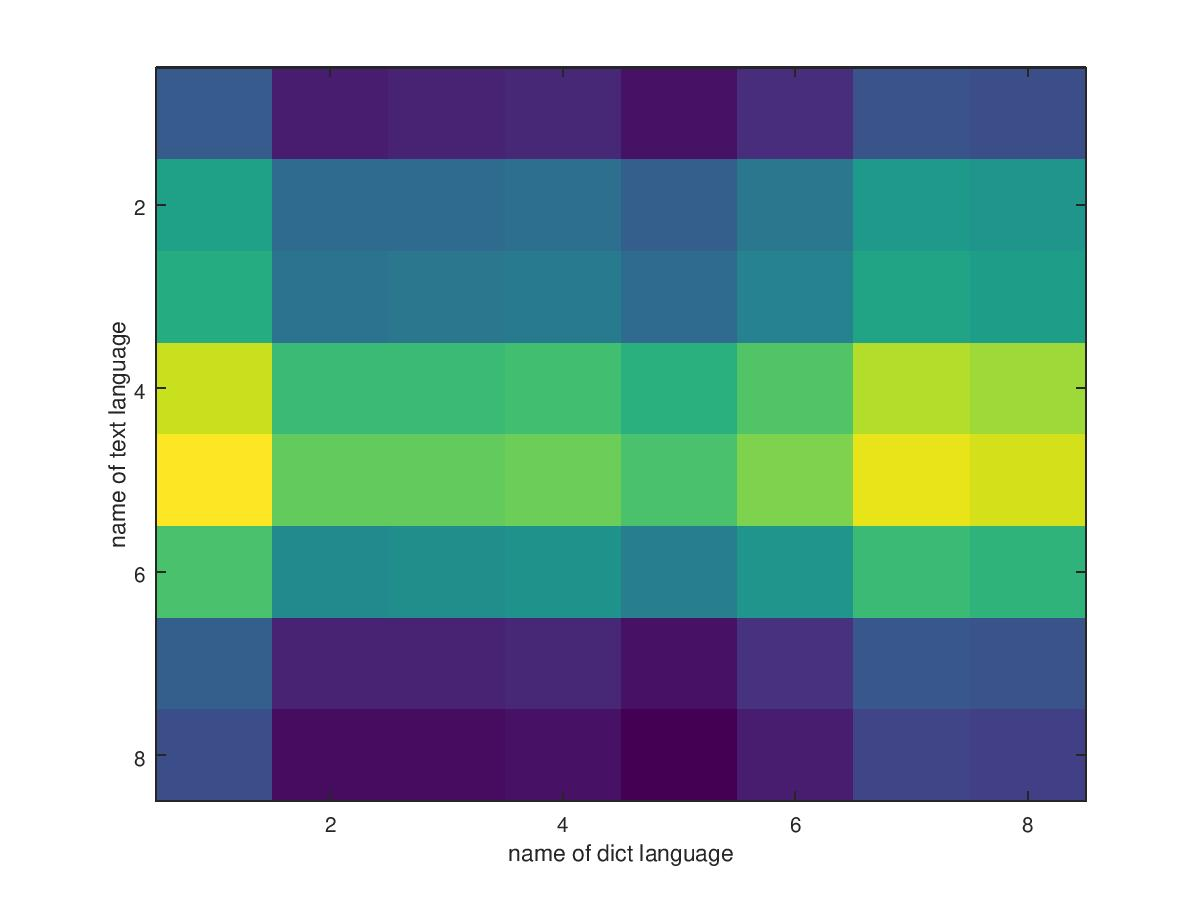
\includegraphics[width=2.5cm]{../images/googleData/witzData.jpg} \\
    \hline
    Witz &
    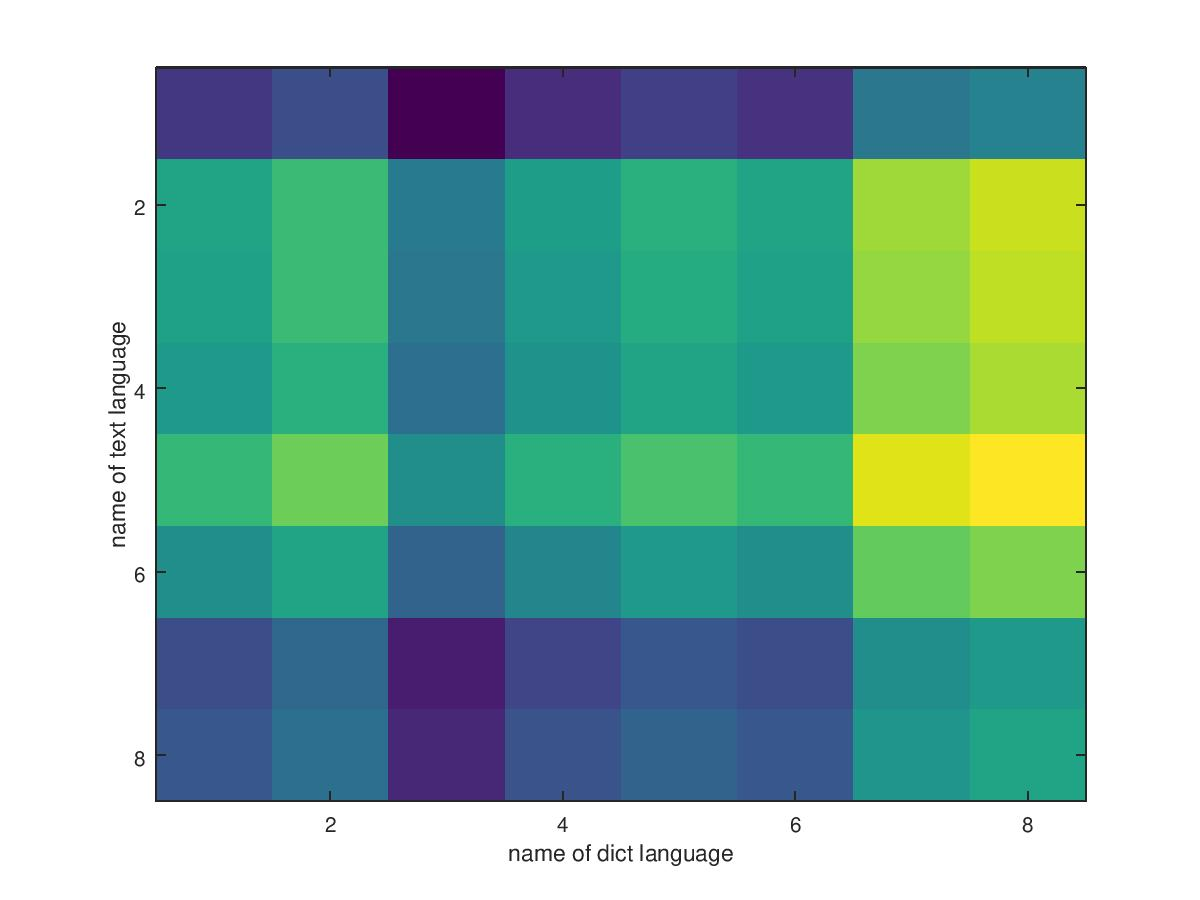
\includegraphics[width=2.5cm]{../images/witzData/abstractData.jpg} &
    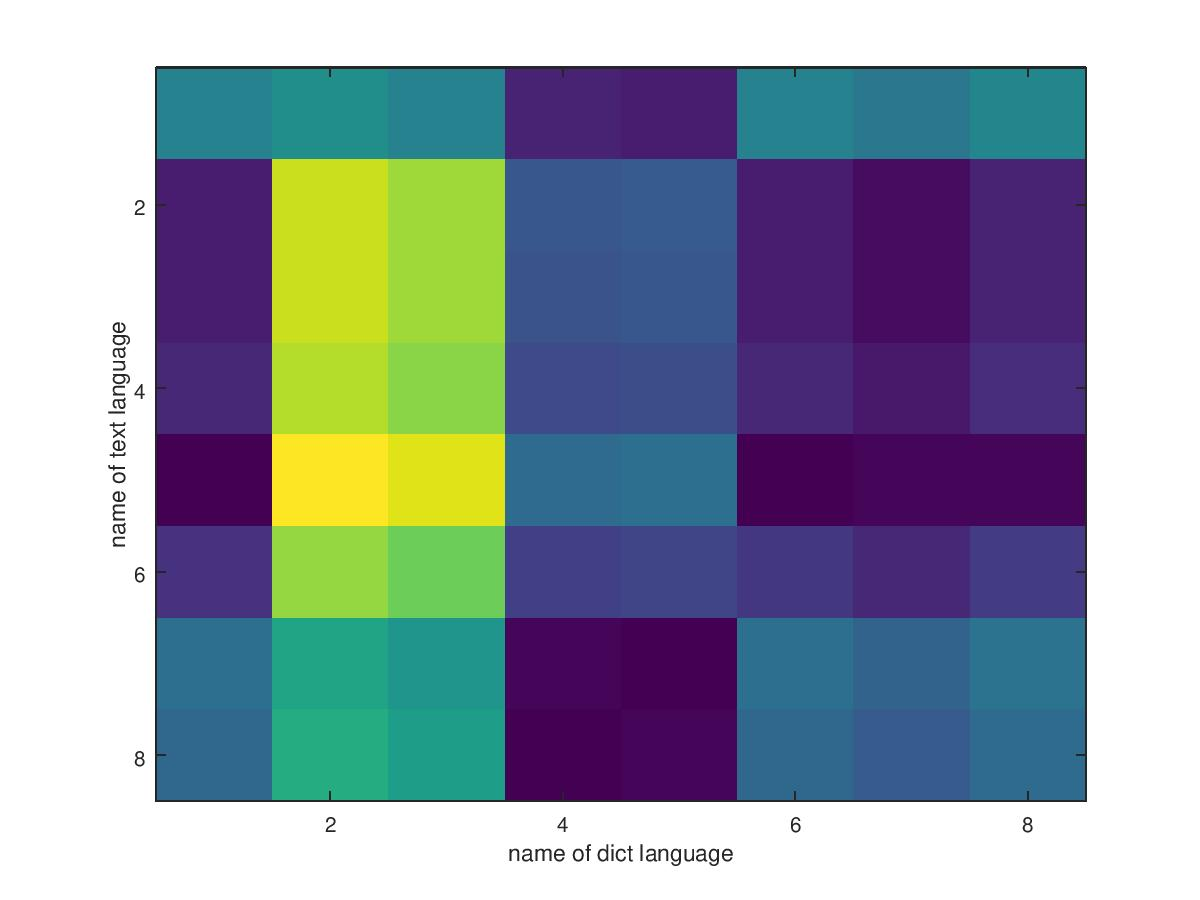
\includegraphics[width=2.5cm]{../images/witzData/dictData.jpg} &
    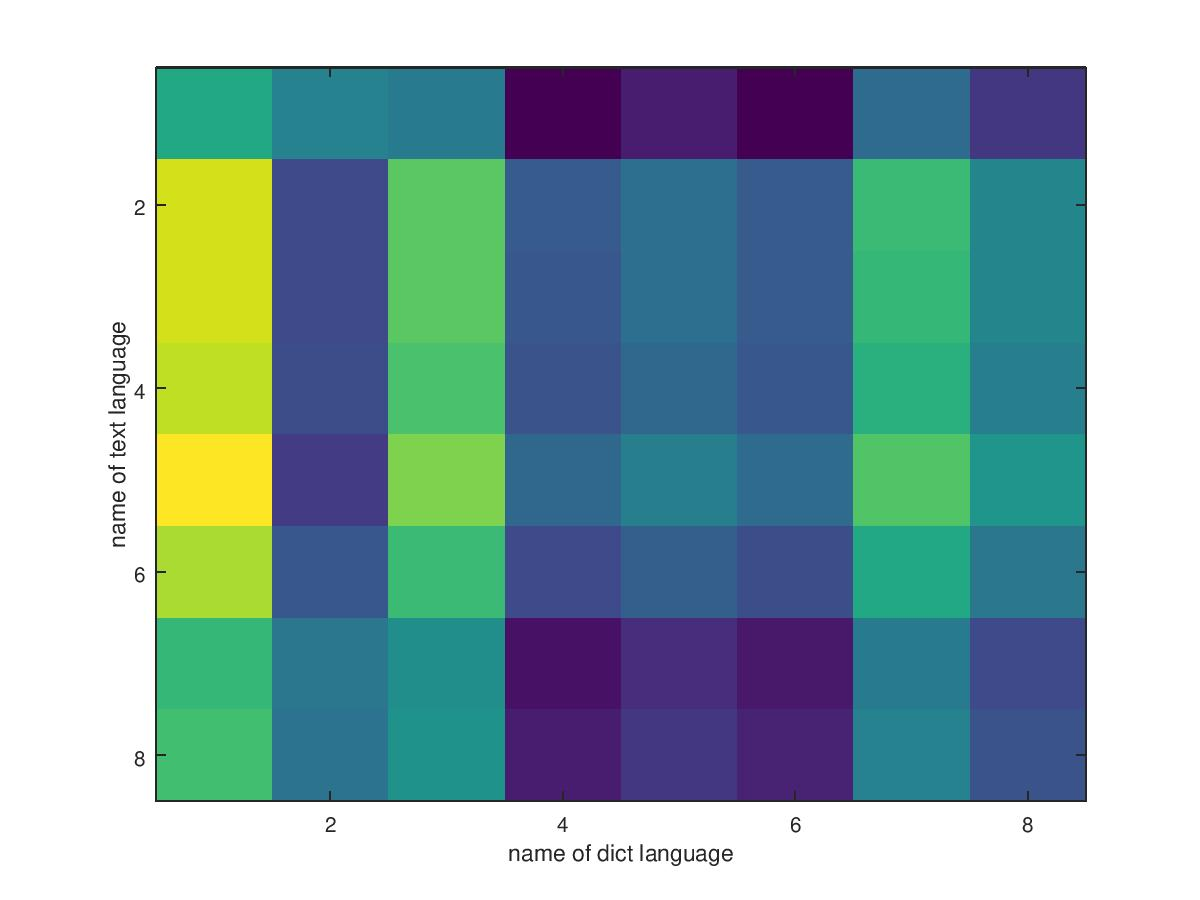
\includegraphics[width=2.5cm]{../images/witzData/facebookData.jpg} &
    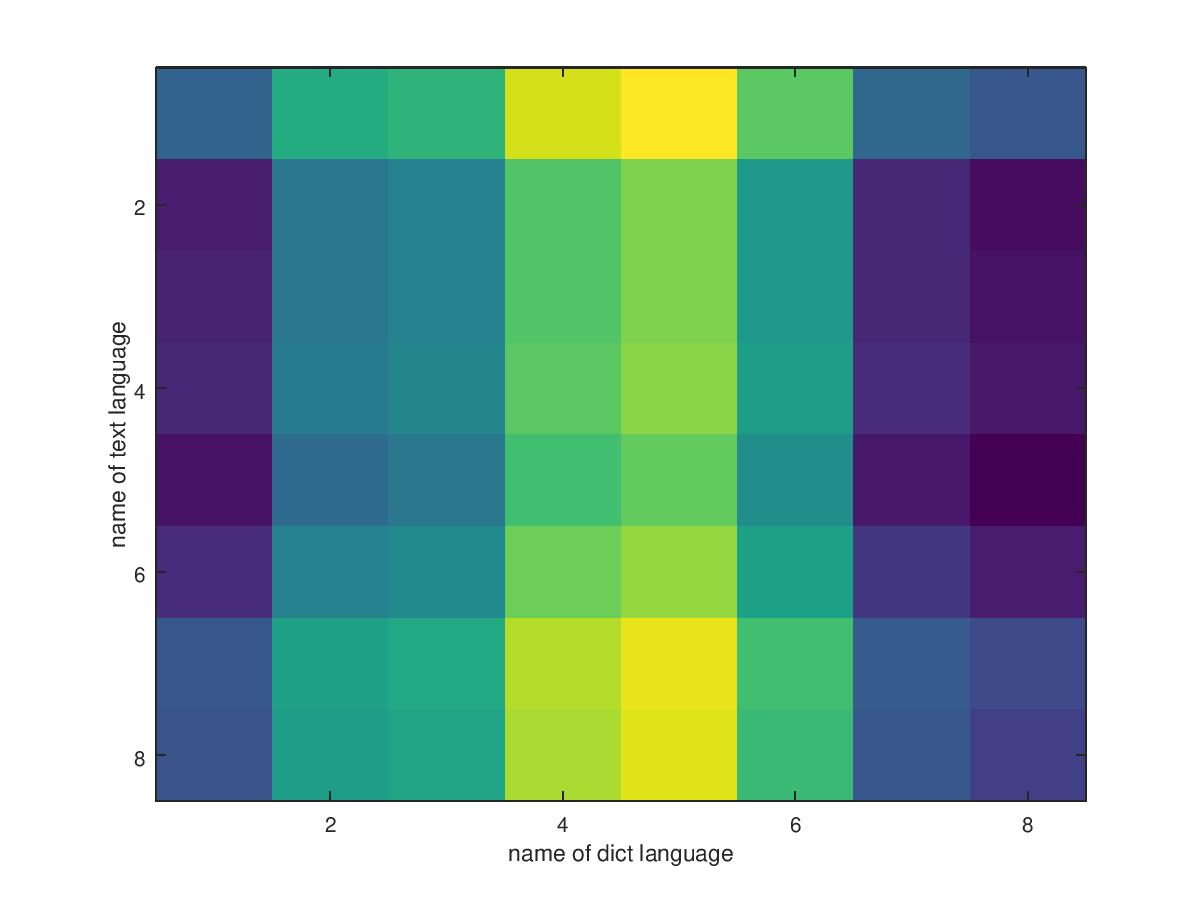
\includegraphics[width=2.5cm]{../images/witzData/googleData.jpg} &
    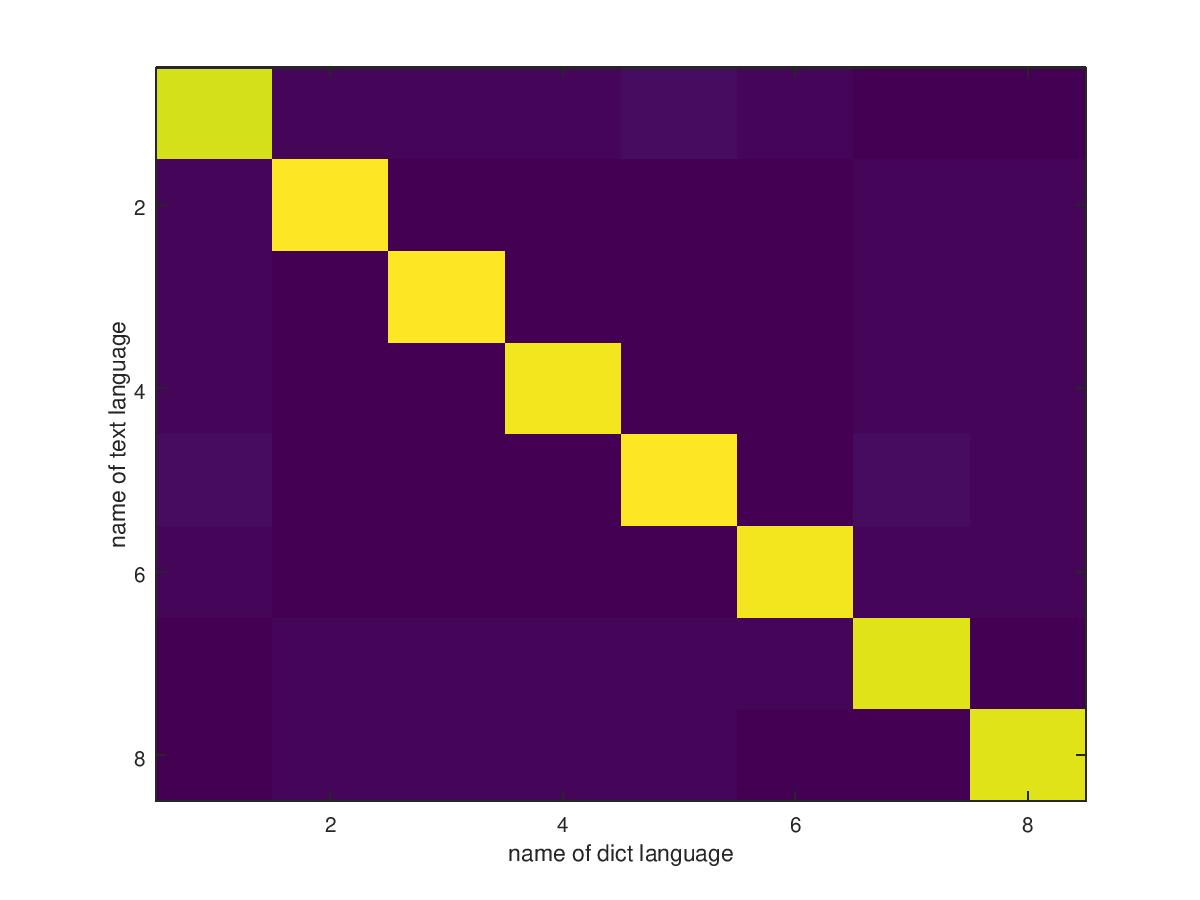
\includegraphics[width=2.5cm]{../images/witzData/witzData.jpg} \\
    \hline
  \end{tabular}
  \caption{Auswertung der Datensätze}
  \label{tab:datenAuswertungText}
\end{table}


Eine Datenauswertung wie in Table \ref{tab:datenAuswertungText} lässt deutlich erkennen, dass trivialer Weise eine Symmetrie um die Diagonale besteht und Laufzeit gespart werden könnte wenn diese ausgenutzt würde. In unserer Implementierung wurde darauf aber nicht geachtet. 


\begin{figure}[H]
	\centering
	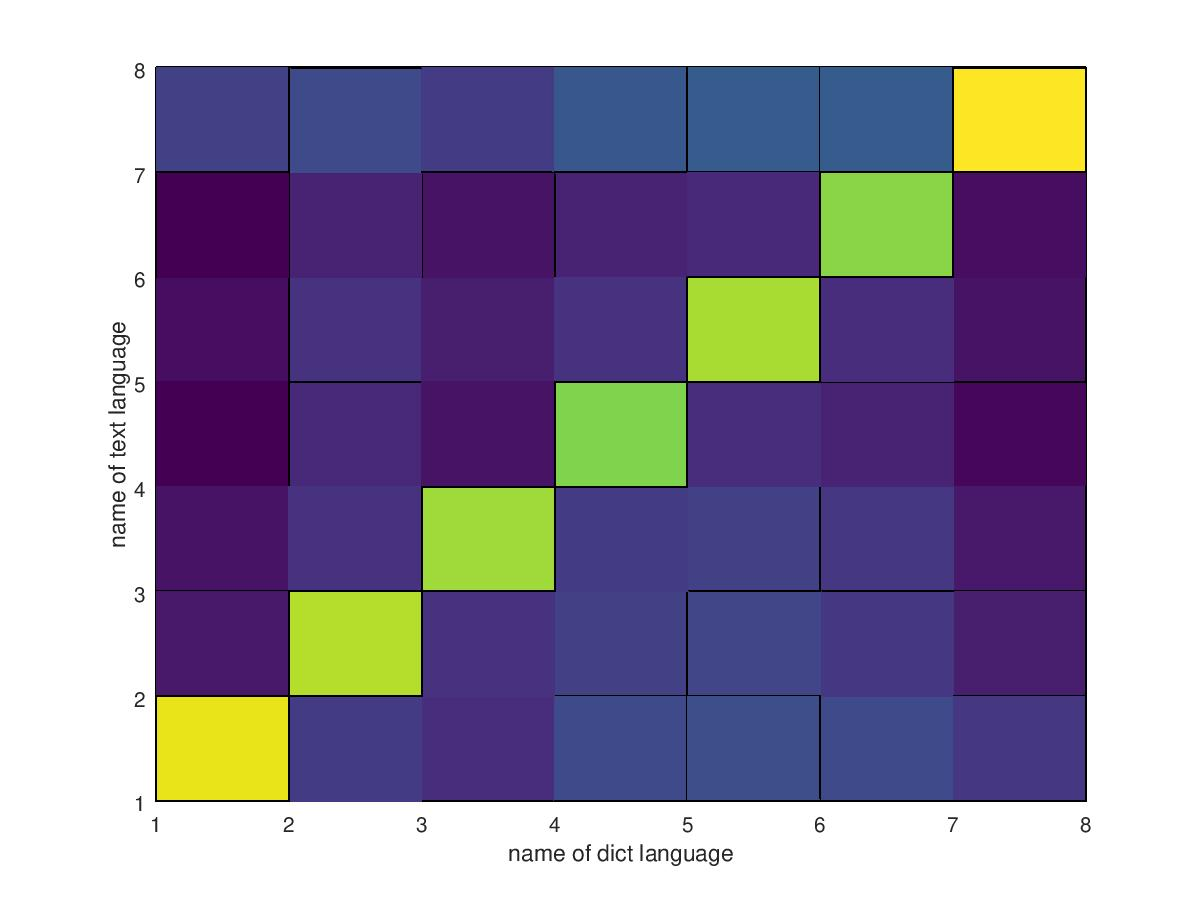
\includegraphics[width=12cm]{images/resultZipData.jpg}
	\caption{zipDataMatrix}
	\label{fig: zipDataMatrix}
\end{figure}

\newpage
\lstinputlisting[frame=single,language=MATLAB,breaklines=true,caption = Octave Script zur Darstellung der einzelnen Kompressionsraten.]{../calculateZipMatrix.m}
\label{fig: calculateMatrixOctaveCode}


\subsection{Kompression und Code-Transformation}
\subsubsection{Lempel-Ziv-Welch Kompression einer Sequenz}
Figure \ref{fig: manualLemperZivPdf} zeigt die händische Berechnung der Lempel-Ziv-Welch Kompression. Beim Übertragen ins Protokoll wurde allerdings ein Fehler entdeckt, der in Tabelle \ref{tab:Level Ziv Kompression} korrigiert wurde.



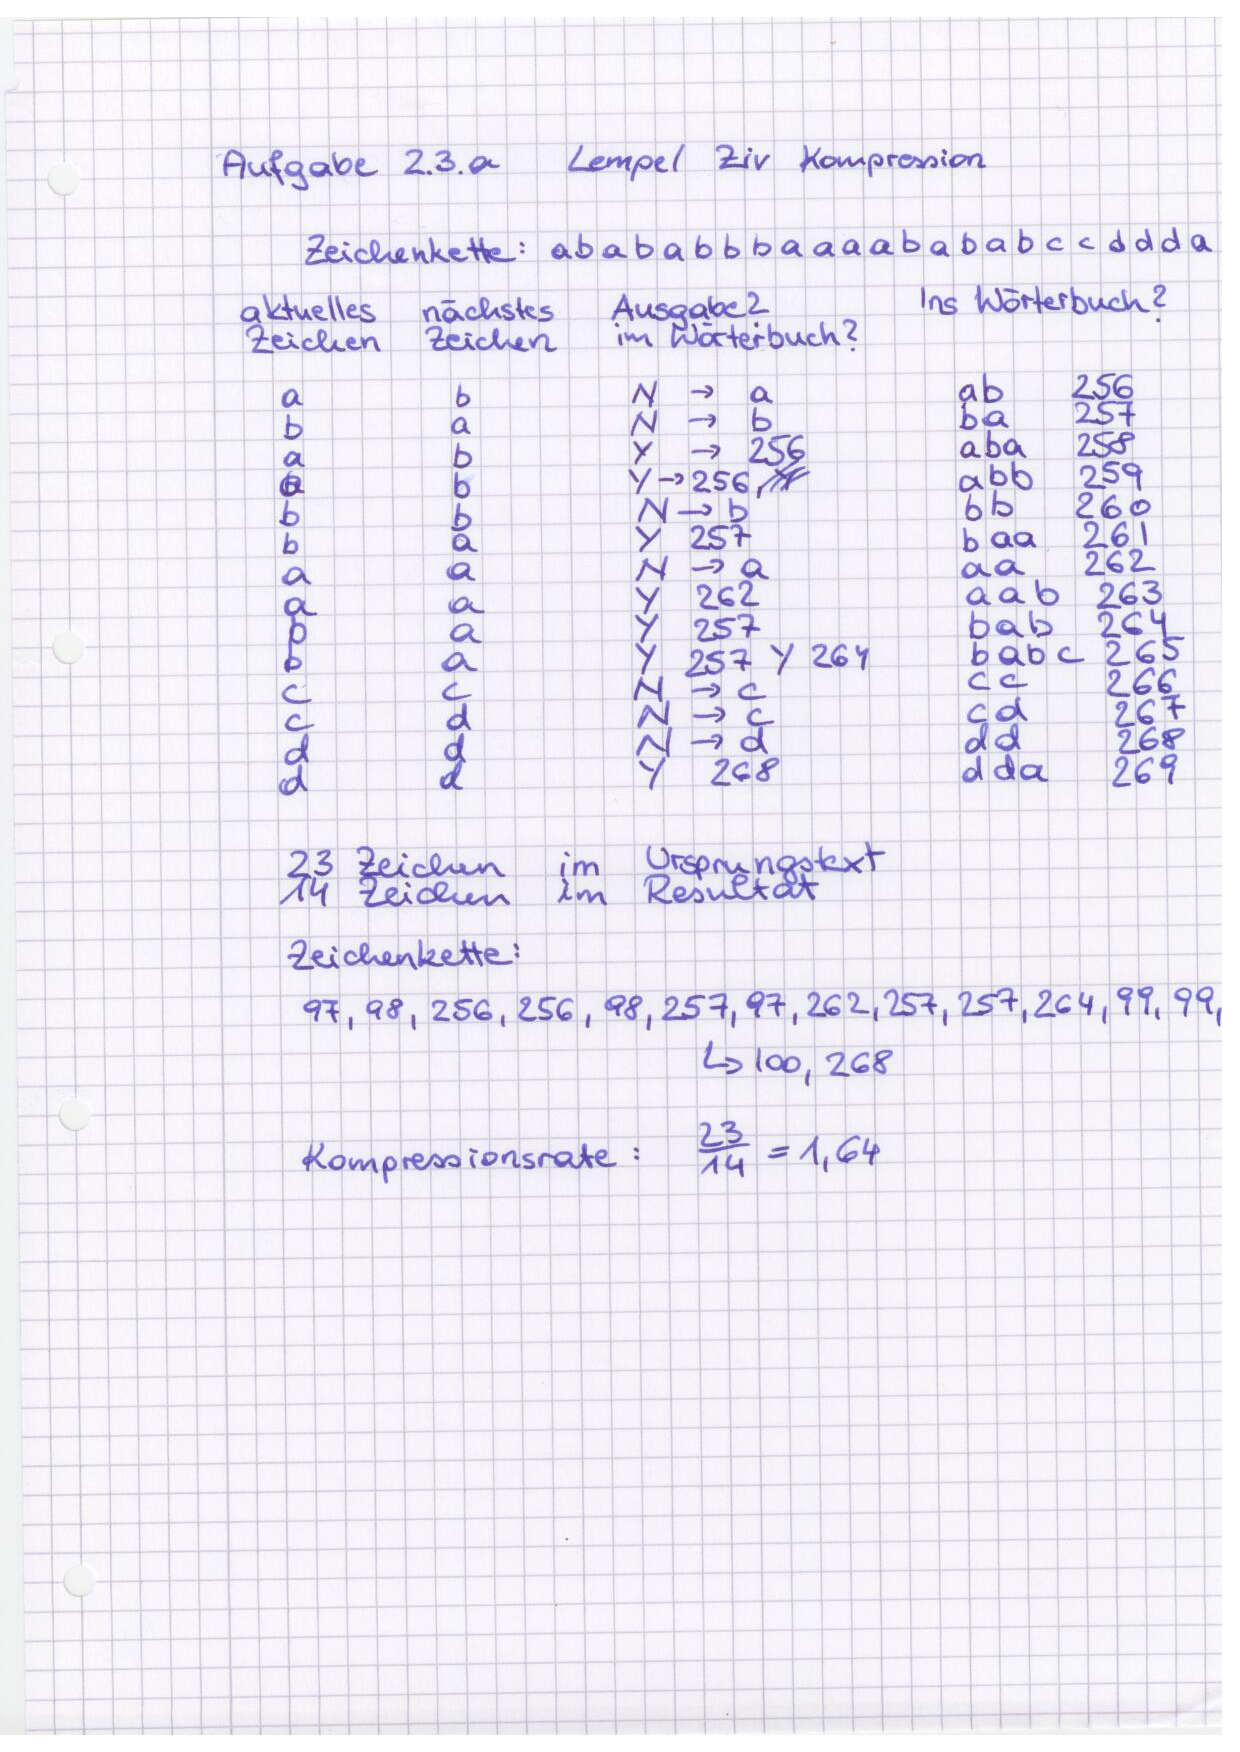
\includepdf[scale=0.4]{images/lemperZiv.pdf}
\label{fig: manualLemperZivPdf}


\begin{table}[H]
  \centering
  \begin{tabular}{| c | c | c | c | c |}
    \hline
   	aktuelles  & nächstes  & Ausgabe  & ins & Speicher \\
   	 Zeichen &  Zeichen &  (im Wörterbuch?) & Wörterbuch! &  \\
	a & b & N $ \rightarrow $ a & ab & 256 \\
	b & a & N $ \rightarrow $ b & ba & 257 \\
	a & b & Y $ \rightarrow $ 256 & aba & 258 \\
	a & b & Y $ \rightarrow $ 256 & abb & 259 \\
	b & b & N $ \rightarrow $ b & bb & 260 \\
	b & a & Y $ \rightarrow $ 257 & baa & 261 \\
	a & a & N $ \rightarrow $ a & aa & 262 \\
	a & a & Y $ \rightarrow $ 256 & aab & 263 \\
	b & a & Y $ \rightarrow $ 257 & bab & 264 \\
	b & a & Y (257), Y $ \rightarrow $ 264 & babc & 265 \\
	c & c & N $ \rightarrow $ c & cc & 266 \\
	c & d & N $ \rightarrow $ c & cd & 267 \\
	d & d & N $ \rightarrow $ d & dd & 268 \\
	d & d & Y $ \rightarrow $ 268 & dda & 269 \\
	a &   & N $ \rightarrow $ a &     &   \\ 
   	
  \end{tabular}
  \caption{Level Ziv Kompression}
  \label{tab:Level Ziv Kompression}
\end{table}

In der korrigierten Version ergibt die resultierende Zeichenkette: 

\begin{table}[H]
  \centering
  \begin{tabular}{| c | c | c | c | c | c | c | c | c | c | c | c | c | c | c |}
    \hline
    97 & 98& 256 & 256 & 98 & 257 & 97 & 262 & 257 & 264 & 99 & 99 & 100 & 268 & 269 \\
    \hline
  \end{tabular}
\end{table}


\begin{equation}[H]
 Kompressionsrate C = \frac{23}{15} = 1.5334	
\end{equation}


\subsubsection{Huffmann Coding}

Die nächste Seite zeigt die händische Berechnung des Huffmann Baums zum gegebenen Beispiel. Die mittlere Codewortlänge liegt dabei bei $1.869 bit $. \\

Weiters kann man auf der darauffolgenden Seite die manuelle Berechnung von 6 Testfällen finden. Es kann gesagt werden, dass die Huffmann Kompression sehr gut geeignet wäre um Daten zu komprimieren, die sehr oft gleich sind. Dabei spielt Homogenität keine Rolle, sondern rein die Häufigkeit des Auftretens der Sonderfälle. An dieser Stelle sei erwähnt, dass die Information über solche Sonderfälle nicht verloren geht, sondern einfach mehr Speicher benötigt wird (verlustfreies Komprimieren).

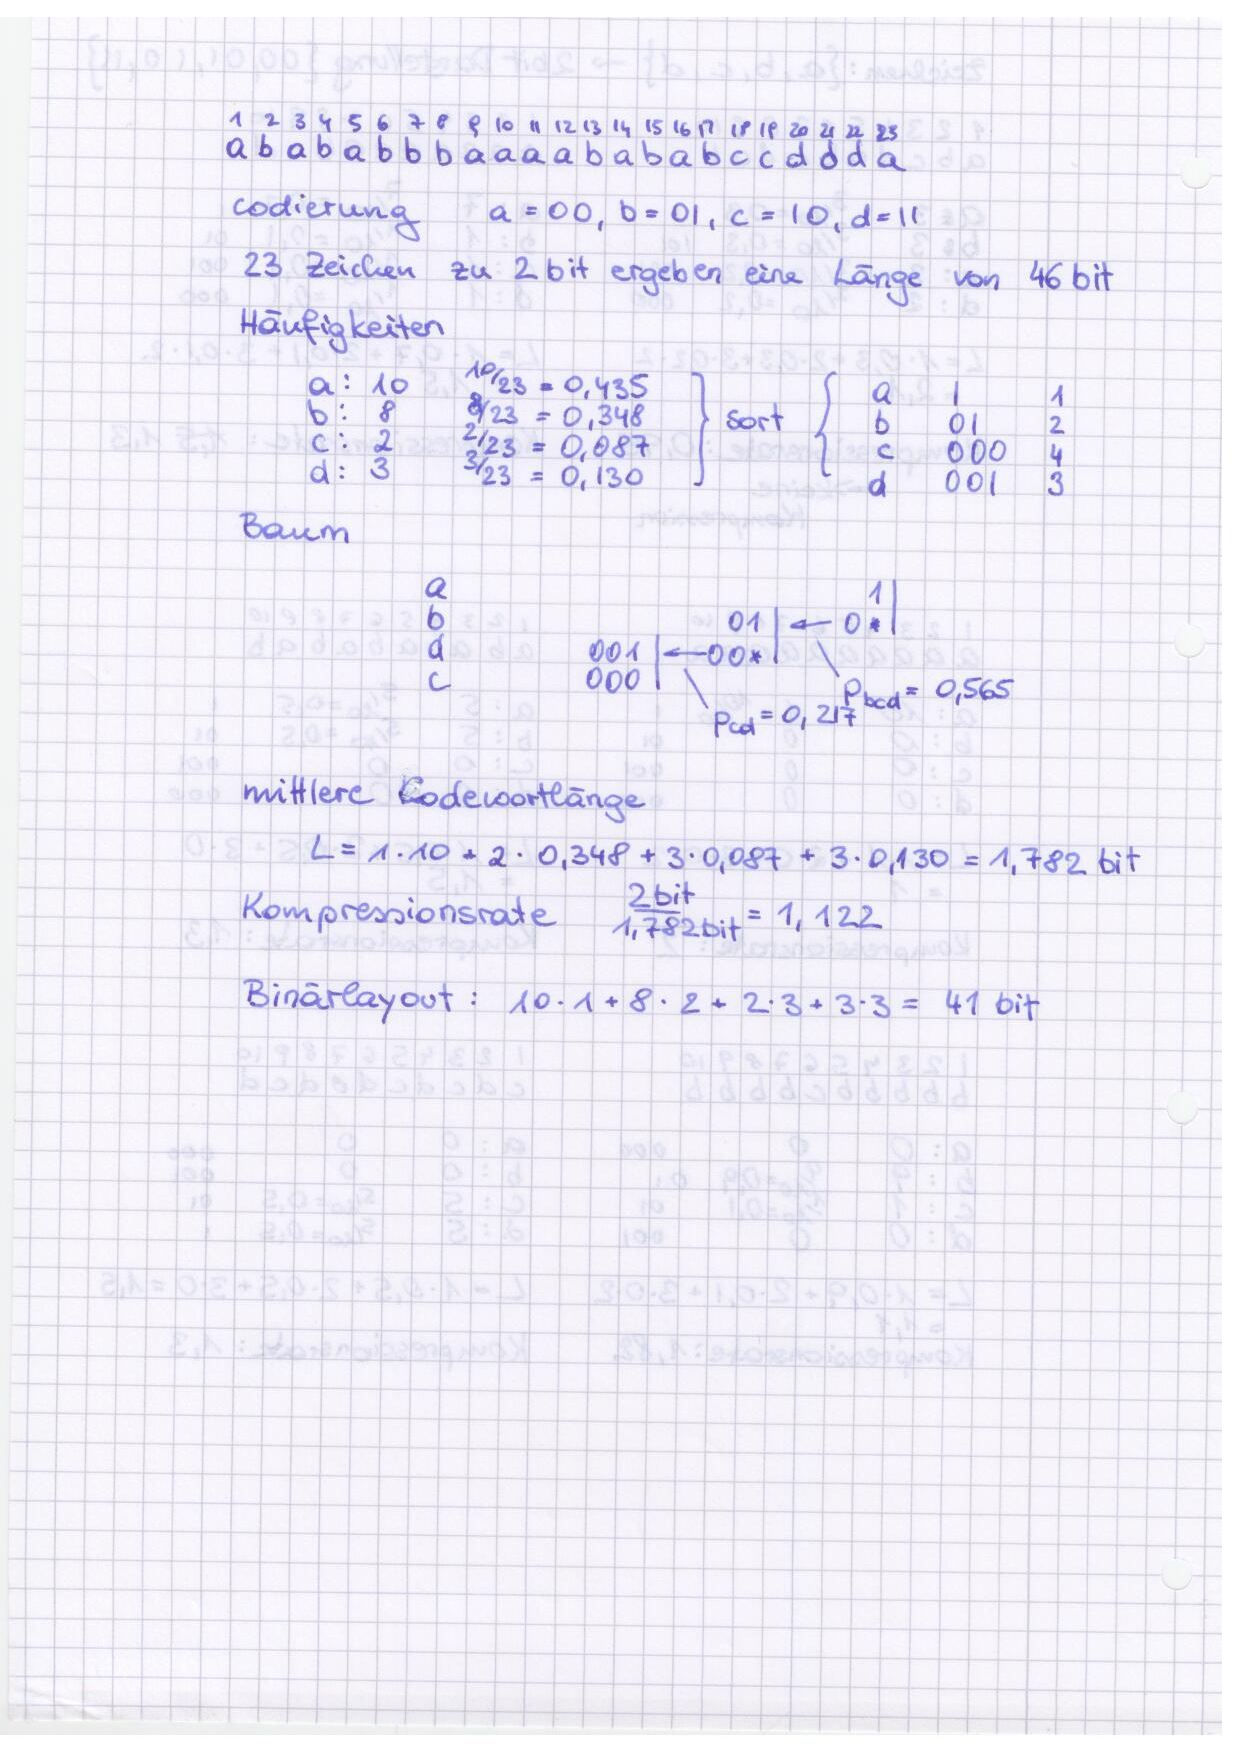
\includepdf{images/huffmannBerechnung.pdf}
\label{fig:huffmannCalculation}

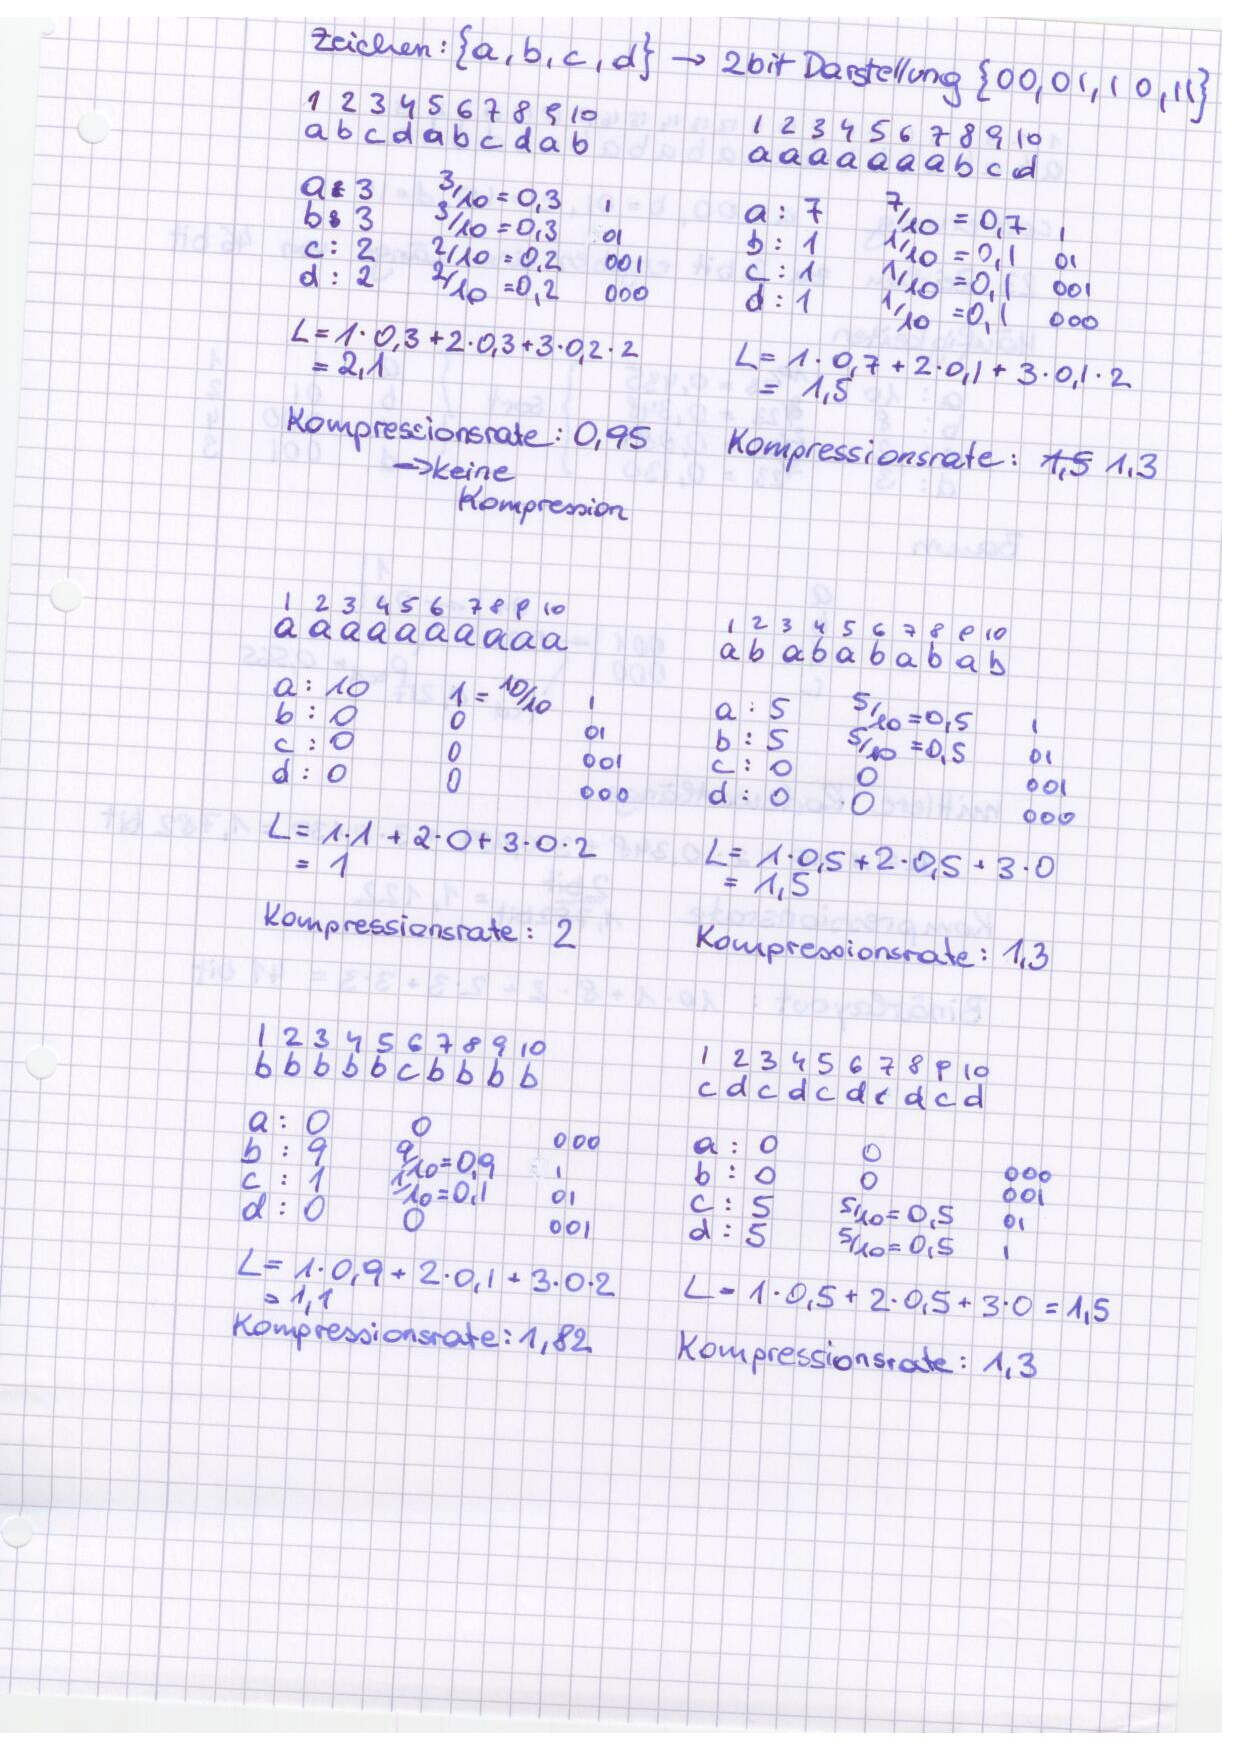
\includepdf{images/huffmannTestfaelle.pdf}
\label{fig:huffmannCalculation}


\subsubsection{Komprimierung einer Sequenz mittels Runlength Coding}
\textit{Berechnung der Kompressionsrate} 

Die nachfolgende Sequenz soll anhand von Runlength Coding händisch komprimiert und die Kompressionsrate ausgegeben werden:

010101111100000111100010101111 (30 Stellen, n=2 Symbole:0,1) \\

Die Sequenz wird von links nach rechts codiert, und anstatt der eigentlichen Zeichen die Häufigkeit dieser ausgegeben. Nach der händischen Komprimierung weist die Frequenz folgende Lauflänge auf:

11111554311114 (14 Stellen)\\


Daraus ergibt sich folgende Kompressionsrate:

30/14 = \textbf{ 2,14}\\

\textit{Erweiterung der Symbolmenge}\\
Die Komprimierung von Sequenzen anhand der RLC ist am effektivsten, je homogener der Informationsgehalt ist. Das bedeutet, das bei vielen unterschiedlichen Zeichen die Komprimierungsmethode nicht mehr sinnvoll angewandt werden kann. Bei sehr kurzen Sequenzen kann es sogar zu einer Erhöhung der Zeichenanzahl in dieser kommen.\\

Wird nun die Anzahl der Symbole erhöht, muss beachtet werden, dass zusätzlich zu der Häufigkeit des Zeichens noch ein Trennsymbol, eine ID bzw. das Zeichen selbst mitgegeben werden muss. Dies wird anhand eines selbst gewählten Beispiels demonstriert.\\

Folgende Sequenz wird anhand von RLC komprimiert:

AAZZBBBBBBBBCCCCCCCDEEEEEEEFFGHIIJJJKLMN\\ (40 Stellen, n=14 Symbole:A,Z,B,C,D,E,F,G,H,I,J,K,L,M,N)\\

Die komprimierte Sequenz lautet:

A2Z2B8C7D1E7F2H1I2J3K1L1M1N1 (28 Stellen)\\

Daraus ergibt sich folgende Kompressionsrate:

40/28=\textbf{1,42}\\

Wird eine sehr kurze Sequenz mit einer hohen Anzahl an Symbolen komprimiert, kann es aufgrund des hohen Informationsgehalts dazu kommen, dass die codierte Sequenz länger ist, als die Originale.\\


Folgende Sequenz wird anhand von RLC komprimiert:

AZBBCDEEFFFGHIIJJJKLLLMNOPQRSTU\\ (30 Stellen, n=21 Symbole:A,Z, B,C,D,E,F,G,H,I,J,K,L,M,N,O,P,Q,R,S,T)\\

Die komprimierte Sequenz lautet:

A1Z1B2C1D1E2F3G1H1I2J3K1L3M1N1O1P1Q1R1S1T1 (42 Stellen)\\

Daraus ergibt sich folgende Kompressionsrate:

30/42=\textbf{0,71}\\

\subsubsection{Entropieberechnung}
Folgende Sequenz zur Entropieberechnung ist gegeben:

111122661112233334564511211111 (30 Stellen, n=6 Symbole: 1,2,3,4,5,6)\\

\begin{figure}[H]
	\centering
	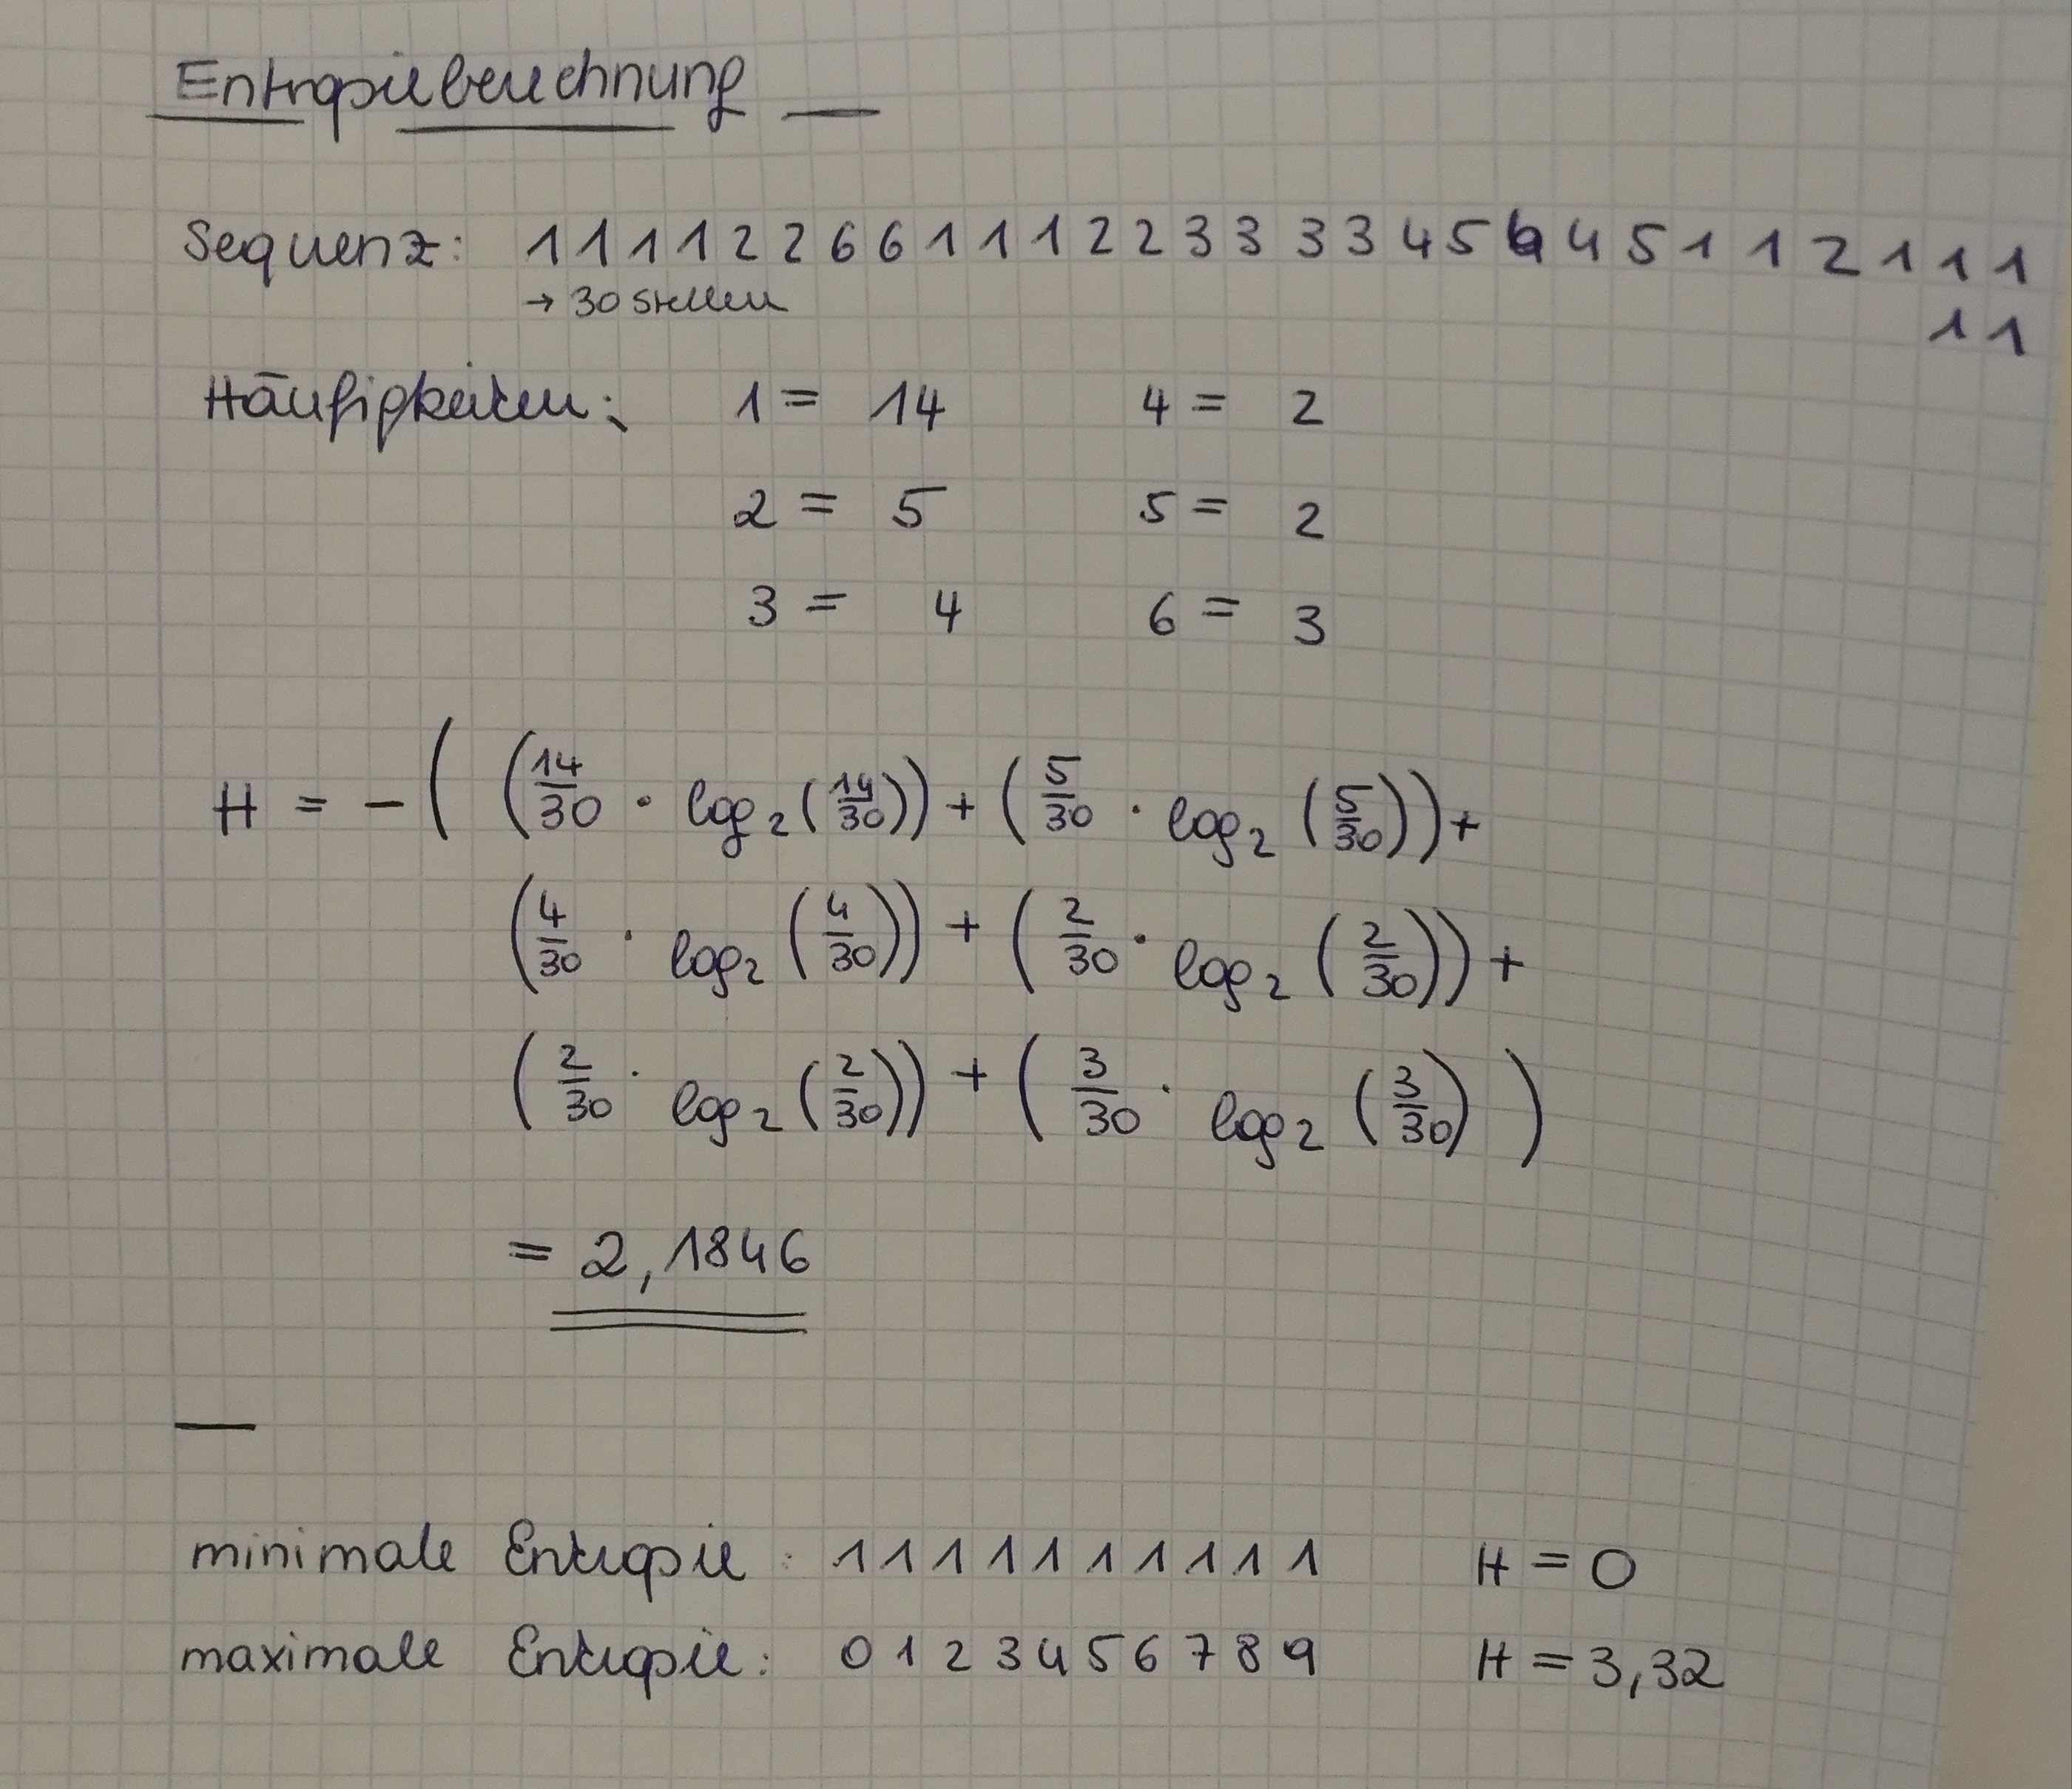
\includegraphics[width=12cm]{images/entropieBerechnung.jpg}
	\caption{manuelle Entropieberechnung}
	\label{fig:resultEntropie}
\end{figure}

Nachdem die Häufigkeiten der Symbole erfasst wurde, wurde die Formel der Shannon-Entropie angewandt. Das Ergebnis der Berechnung lautet \textbf{2,1846}. \\

\textit{Minimale und Maximale Entropie}

Bei foglender 10-stelliger Sequenz ist die Entropie minimal:

Sequenz: 1111111111 (10 Stellen, n=1 Symbol: 1)

H = 0\\

Bei folgender 10-stelliger Sequenz ist die Entropie maximal:

Sequenz: 0123456789 (10 Stellen, n=10 Symbole: 0,1,2,3,4,5,6,7,8,9)

H = 3,32\\

\textit{Auswirkung auf Kompressionsrate}\\

Eine geringe Entropie bewirkt, dass die Sequenz besser komprimierbar ist.  Je höher die Entropie, desto schlechter ist die Sequenz komprimierbar. Nicht nur die Auftrittswahrscheinlichkeit hat eine Auswirkung auf die erzielbare Kompressionsrate. Auch die Länge der Sequenz, sowie die Anzahl der Zeichen spielt eine wesentliche Rolle. Je größer diese Faktoren, desto schlechter ist eine Sequenz durch unterschiedliche Kompressionsverfahren bearbeitbar.



\end{document}
